\documentclass[11pt]{article}

% ============================================================
% ACL FORMAT
% ============================================================

% Use [review] for anonymous review version.
% For the final/camera-ready version, use:
% \usepackage{acl}
\usepackage{acl}

\usepackage{times}
\usepackage{latexsym}
\usepackage[T1]{fontenc}
\usepackage[utf8]{inputenc}
\usepackage{microtype}
\usepackage{inconsolata}
\usepackage{amsmath}

\usepackage{graphicx}
\usepackage{booktabs}
\usepackage{subcaption}


\title{Toward Personalized Hebrew ASR: Adapting a General Model to a Single Speaker}

\author{
  Dolev Abudi \\
  Tel Aviv University \\
  \texttt{dolevabudi@mail.tau.ac.il} \\\And
  Hadas Yonat \\
  Tel Aviv University \\
  \texttt{hadasyonat@mail.tau.ac.il}
}

\begin{document}

\maketitle

% NOTE: The paper is limited to 5 pages excluding references and appendices.
% Rough budget: abstract + introduction ~1 page, experimental setup ~1.5 pages,
% results ~2 pages, conclusion + limitations ~0.5 page.


% ============================================================
% ABSTRACT
% ============================================================

\begin{abstract}
Automatic speech recognition (ASR) systems are built for general-purpose use
and evaluated by error rates averaged across many speakers, which says little
about how well they serve any one person. Yet in many deployments it is a single
speaker's accuracy that matters. We ask how to personalize a Hebrew ASR model to
one speaker under a small data and compute budget.
% TODO: Complete the abstract once results are final:
% (3) what we did (speaker-level diagnosis on VoxKnesset, then per-speaker
%     and per-subgroup adaptation of a Hebrew Whisper model),
% (4) headline results,
% (5) what this means.
\end{abstract}


% ============================================================
% INTRODUCTION
% ============================================================

\section{Introduction}

Modern ASR models such as Whisper \citep{radford2023whisper} are built for
general-purpose use. Their quality is reported as an error rate averaged over
many speakers and corpora, an average that can hide large differences: a model
that serves most people well may still serve some of them poorly.

In many real deployments, however, the user is not the average speaker but one
particular person: a Knesset member whose speeches are transcribed every day, a
journalist dictating notes, or the single user of a voice assistant. For them,
what matters is how well the model recognizes their own voice. This calls for
personalization: adapting a general model to one speaker with a small amount of
their own speech.

We study personalization for Hebrew and ask four questions: which fine-tuning
strategy suits a single speaker, how much of their speech is needed, who
benefits most, and whether a personal model outperforms one shared across
speakers.

% TODO: Complete the introduction once results are final:
% - Contributions: a practical recipe for personalizing Hebrew ASR, a
%   comparison of personal against shared adaptation, and the first
%   speaker-level error map for Hebrew recognition.
% - Footnote with the code/artifact link.


% ============================================================
% RELATED WORK
% ============================================================

\section{Related Work}

\paragraph{Averages hide who is served.}
Whisper \citep{radford2023whisper} and ivrit.ai's Hebrew model
\citep{marmor2025hebrewasr} are both evaluated by error rates averaged over
large test sets, never per speaker or subgroup. Such averages have hidden gaps
before: Whisper is much weaker on languages with little training data, Hebrew
among them. ivrit.ai closed this language gap by fine-tuning Whisper on about
5{,}000 hours of Hebrew, mostly Knesset plenary speech, producing
\texttt{ivrit-ai/whisper-large-v3}, the starting point for our work.

\paragraph{Gaps within a language.}
Within a single language, too, ASR serves some people worse than others. Error
rates differ by race \citep{koenecke2020racial} and by gender, dialect, age and
accent \citep{tatman2017gender,feng2021quantifying,liu2022fairness}. These
studies compare groups, and we are not aware of such an analysis for Hebrew. We
close this gap on the analysis side: we measure the error, and the gain from the
Hebrew fine-tune, for each speaker and for subgroups of speakers who share
attributes such as gender, age, origin or speaking rate.

\paragraph{Adapting a model to one speaker.}
Adapting a recognizer to its user is an old idea in speech recognition
\citep{gales1998mllr}. With modern models, fine-tuning on a small amount of a
person's own speech can greatly reduce their errors, but this has mostly been
studied for atypical speech, such as speech impairments and strong accents
\citep{shor2019personalizing,green2021disordered}. Training a full model for
every speaker is expensive, so methods such as LoRA \citep{hu2022lora} train only
a small number of added parameters, and have also been used with Whisper
\citep{liu2024s2lora}.


% ============================================================
% EXPERIMENTAL SETUP
% ============================================================
\section{Experimental Setup}


% ------------------------------------------------------------
\subsection{Overview}

Our study consists of two experiments.

In the first experiment, we conduct a speaker-level performance analysis, and repeat it for subgroups of speakers who share attributes such as gender, age, origin or speaking rate. Both models transcribe the same held-out speech, allowing us to measure transcription error for each speaker and each subgroup. Because the second model is a Hebrew fine-tuned version of the first, we can also quantify the improvement attributable to Hebrew fine-tuning, per speaker and per subgroup.

In the second experiment, we focus on adaptation. From the speaker-level map, we select 12 speakers covering four profiles: speakers the Hebrew fine-tune helped least, speakers who remain hard under both models, typical speakers, and a low-WER speaker, plus two high-gain speakers as controls. To avoid selecting on measurement noise, speakers are ranked on their earlier sessions only, and their newest sessions are held out for testing. We then fine-tune the Hebrew model on each speaker's own speech, and compare it with a control adapter trained on the same amount of speech pooled from other speakers. This separates learning the individual voice from learning committee speech in general.


% ------------------------------------------------------------
\subsection{Data}
\label{sec:data}

We use \texttt{ivrit-ai/knesset-committees}, a corpus of Israeli parliamentary committee sessions built from recorded audio--video and human-written protocols. The protocols are aligned to the recordings using forced alignment, providing transcript segments with speaker identities and alignment-confidence scores. Since the protocols are stenographic rather than fully verbatim, low-confidence segments may reflect mismatches between the text and audio.

The corpus spans November 2018 to January 2026 and contains approximately 13{,}177 sessions and 15{,}466 recorded hours, including about 7{,}886 hours of aligned speech with confidence scores above 0.7.


% ------------------------------------------------------------
\subsection{Models}
\label{sec:models}

We compare two models that share Whisper's encoder--decoder architecture and
differ in language-specific adaptation.
Arm~\textbf{A} is \texttt{openai/whisper-large-v3} \citep{radford2023whisper},
the general multilingual model, and arm~\textbf{B} is
\texttt{ivrit-ai/whisper-large-v3} \citep{marmor2025hebrewasr}, the same model
after fine-tuning on roughly 4{,}700 hours of Hebrew
\emph{plenary} speech.
Arm~B is also the starting point for personalization: all speaker and subgroup
adaptation further fine-tunes \texttt{ivrit-ai/whisper-large-v3}.
For the speaker-level analysis, arm~B is served through ivrit.ai's inference
checkpoint (\texttt{whisper-large-v3-turbo-ct2}, with 4 decoder layers instead of 32).

% ------------------------------------------------------------
\subsection{Preprocessing}
\label{sec:preprocessing}

The corpus \texttt{ivrit-ai/knesset-committees} cannot be used directly in its released form. Whisper processes audio in segments of at most 30 seconds, whereas committee sessions can last several hours. In addition, our analysis is speaker-level, so each segment must be linked to a verified individual.

We therefore follow the preprocessing procedure introduced by VoxKnesset \citep{marmor2026voxknesset}, a 2{,}300-hour corpus of Hebrew parliamentary speech from 393 Knesset members with verified speaker identities and demographic metadata. We do not use VoxKnesset audio itself because it comes from the very plenary sessions arm~B was fine-tuned on, so evaluating on it would test the model on speech it has already seen.

Speaker identification is performed first. Protocol speaker names are matched to the Knesset's official roster of name variants and accepted only when consistent with the member's term of service. Unresolved identities are discarded. During this stage, speaker-level attributes such as birth year, gender, and origin are also joined to the dataset using the matched Knesset member identity.

Each identified speaker turn is then divided into segments of at most 30 seconds without crossing speaker boundaries, with the aligned protocol text used as the reference transcript. Where dataset splits are required, they are session-disjoint within each speaker.

Each segment carries an alignment quality score between 0 and 1, indicating how well its protocol text is aligned to the audio (defined in Appendix~\ref{app:data}). Segments below 0.7 are excluded from all analyses. Training and validation data are further restricted to segments above 0.95, following ivrit.ai's recommendation (Appendix~\ref{app:data}).

% ------------------------------------------------------------
\subsection{Speaker-Level Performance}

To evaluate performance at the speaker level, we run inference with both models on the same set of audio segments: arm~A through Hugging Face Inference Providers and arm~B through a RunPod serverless endpoint hosting ivrit.ai's inference checkpoint. To ensure comparability across speakers, we sample one hour of speech per speaker using a round-robin procedure over their sessions, so that the selected audio spans each speaker's tenure.

For each speaker, we report WER and CER under both models, as well as the adaptation gain,
$\text{WER}_A-\text{WER}_B$,
and the relative gain,
$(\text{WER}_A-\text{WER}_B)/\text{WER}_A$.
We also repeat the analysis across speaker subgroups defined by shared attributes.

% ------------------------------------------------------------
\subsection{Personalization}
\label{sec:personalization}

\paragraph{Speakers and data.}
We adapt the 12 selected speakers. To avoid leakage, each speaker's meetings are
split into training, validation and test sets that share no meeting, with the
newest meetings held out for testing (Appendix~\ref{app:additional}). Each speaker
is trained on 5, 20 and 80 minutes of their own speech. The budgets are nested,
filled from the speaker's most recent training meetings first. Every model is
scored on two test sets from the same held-out meetings (Appendix~\ref{app:data}):
the high-quality segments (\emph{clean test}, median 47 minutes per speaker) and
all segments at quality $\geq 0.7$ (\emph{full test}, median 90 minutes).

\paragraph{Adapter and training.}
We train LoRA adapters \citep{hu2022lora} of rank 8 on the query and value
projections of every attention layer of arm~B (3.9M trainable parameters), for at
most 400 steps with early stopping: validation loss is measured every 20 steps on
other meetings of the speaker, used for neither training nor testing, and training
stops after four checks without improvement, restoring the best checkpoint. The
training labels are the protocol text.

\paragraph{Control.}
An adapter trained on a speaker's audio learns both the speaker and the committee
setting: rooms, microphones, vocabulary and the protocol's style. To separate the
two, the 12 speakers are split at random into two folds of six. For each fold and
budget, a \emph{control} adapter is trained with the same recipe on the same
number of minutes from the six speakers of the \emph{other} fold. Each speaker is
scored on the same test segments under their own adapter and under the control,
which never heard them. We report the relative gain over arm~B,
$(\text{WER}_B-\text{WER}_\text{adapted})/\text{WER}_B$, and the
\textbf{personalization},
$(\text{WER}_\text{control}-\text{WER}_\text{own})/\text{WER}_B$, which equals
the own gain minus the control gain. Its 95\% interval and p-value come from a
paired bootstrap over test segments (Appendix~\ref{app:significance}). All budgets
use seed 0; at 80 minutes, seeds 1 and 2 repeat the own adapters and the controls,
with the folds redrawn, to distinguish speaker-level effects from variance caused
by the random seed.


% ============================================================
% RESULTS
% ============================================================

\section{Results}

% TODO: One subsection per finding. Merge or drop subsections if the
% 5-page limit gets tight.

\subsection{Speaker-Level Error Map}
\label{sec:errormap}

\begin{figure}[t]
    \centering
    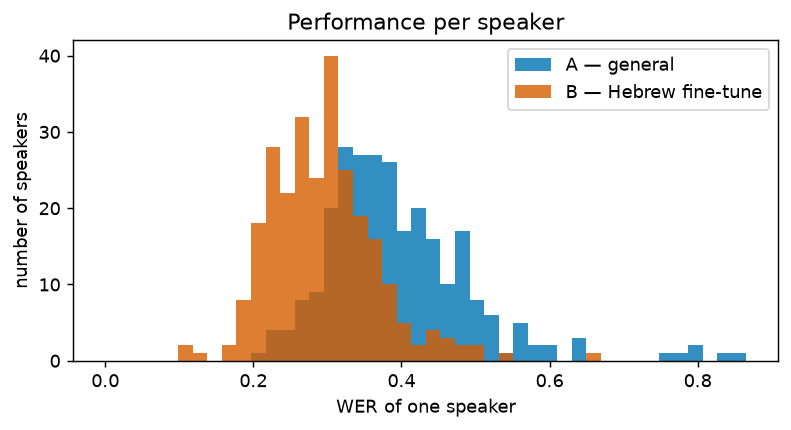
\includegraphics[width=\columnwidth]{figures/error_map_hist.png}
    \caption{Per-speaker WER under arm~A (general) and arm~B (Hebrew fine-tune),
    all 267 speakers. Arm~B shifts the whole distribution down without narrowing it
    in proportion.}
    \label{fig:hist}
\end{figure}

After the quality filter, the analysis covers 267 speakers and 217 hours
(58{,}180 segments), with a corpus WER of 0.387 for arm~A and 0.292 for arm~B.
Statistics below are over the 261 speakers with at least 20 segments, and
per-speaker 95\% confidence intervals come from bootstrapping each speaker's segments
(Appendix~\ref{app:boot-errormap}).

\paragraph{The fine-tune helps every speaker, but not equally.}
All 261 speakers have a lower WER under arm~B, and for every one of them the
improvement is beyond sampling noise: the 95\% bootstrap interval of their gain lies
entirely above zero (Figure~\ref{fig:gain}, Appendix~\ref{app:additional}). Yet the fine-tune does not make speakers more equal (Figure~\ref{fig:hist}): the spread of per-speaker WER
shrinks (standard deviation 0.099 to 0.069) only in proportion to the lower average,
so relative to the mean, speakers differ as much as before (coefficient of variation is 0.25 vs.\ 0.23).
Speakers keep their order (Spearman $\rho=0.90$ between WER$_A$ and WER$_B$),
and this ranking is stable across a speaker's recordings
(Appendix~\ref{app:additional}).

\paragraph{Group membership explains little.}
We compare the gain across seven groupings of speakers: gender, nationality, religion,
religious orientation, country of origin, age quartile and speaking-rate tertile.
The clearest difference is speaking rate (Figure~\ref{fig:rate}, with plots for the other
six groupings in Figure~\ref{fig:groups}, Appendix~\ref{app:additional}): slow speakers gain more than fast ones (27\% vs.\ 22\% of arm~A's error removed). Arab, Muslim, Druze and Bedouin speakers also gain more than
Jewish speakers (29--30\% vs.\ 24\%). However, group sizes are highly imbalanced (e.g., 229 Jewish speakers against 5 Bedouin), and the variation within each group far
exceeds the differences between group medians.
The bottom line: a speaker's group says little about how well the model serves them,
which motivates adapting to individual speakers. We test shared adaptation only on a
randomly pooled group of speakers, and leave further analysis and fine-tuning on demographically defined
subgroups to future work.

\begin{figure}[t]
    \centering
    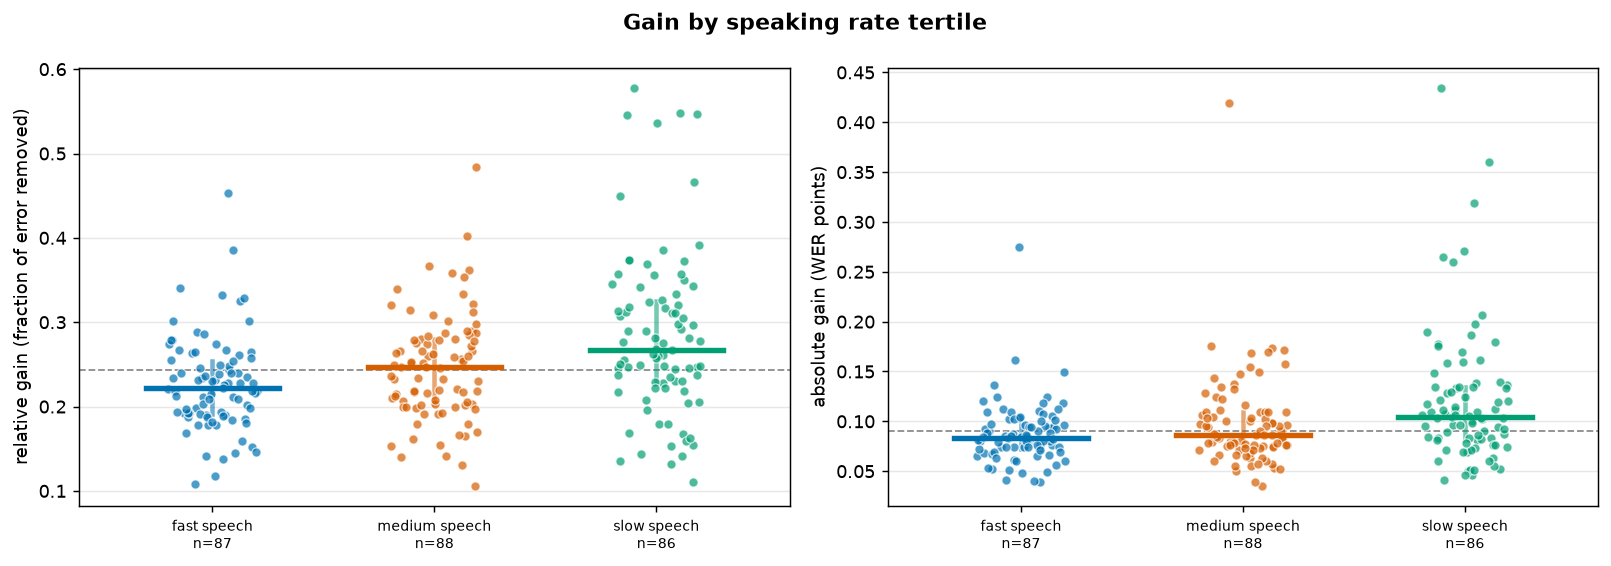
\includegraphics[width=\columnwidth]{figures/group_rate_band.png}
    \caption{Gain from the Hebrew fine-tune by speaking-rate tertile, relative (left) and
    absolute (right). Each point is one speaker, the bar is the group median, and the dashed line is the overall median.}
    \label{fig:rate}
\end{figure}

\paragraph{Speaker selection.}
From this map we select 12 speakers for personalization, covering five profiles:
speakers the Hebrew fine-tune helped least, speakers who remain hard under both models,
typical speakers, a low-WER speaker to test how much headroom is left, and two
high-gain controls.


\subsection{Adaptation Results}
\label{sec:adaptation}

\paragraph{The 80-minute adapter improves almost every speaker.}
In Figure~\ref{fig:budget} (blue, 80 minutes), the own adapter's gain (its relative
WER reduction from arm~B) with seed 0 has a median over the 12 speakers of +12.0\%
on the clean test and +15.3\% on the full test; it is above zero for 11 of 12
speakers on the clean test (9 significantly) and for all 12 on the full test (all
significantly). The other two seeds agree: over all 36 speaker--seed pairs, the
adapter beats arm~B in 35 on the clean test and in all 36 on the full test, and with
each speaker's gain averaged over the three seeds (Figure~\ref{fig:bestmodel},
column ``own 80 min''), the clean-test gains have a median of +11.4\% and a mean of
+13.2\%, ranging from +3\% to +28\%.

\begin{figure}[t]
    \centering
    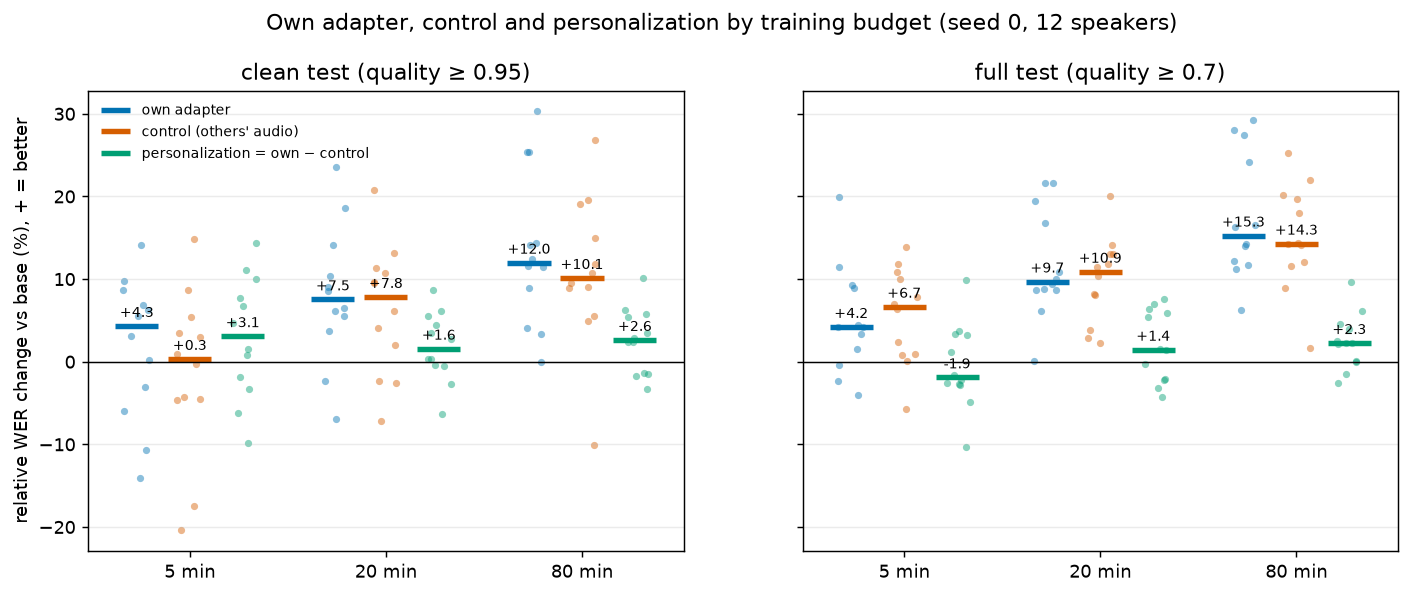
\includegraphics[width=\columnwidth]{figures/stage2_budget_own_control_personalization.png}
    \caption{Relative WER change over arm~B at 5, 20 and 80 minutes of training audio
    (seed 0, 12 speakers), on the clean test (left) and the full test (right). Blue: the
    speaker's own adapter; orange: the control, trained on the same minutes from other
    speakers; green: personalization (own $-$ control). Each dot is one speaker; bars and
    numbers are medians. The median personalization is the median of per-speaker
    differences, not the difference of the two medians.}
    \label{fig:budget}
\end{figure}

% Full width: two heatmaps of 12 speakers x 6 adapters do not read at column width.
\begin{figure*}[t]
    \centering
    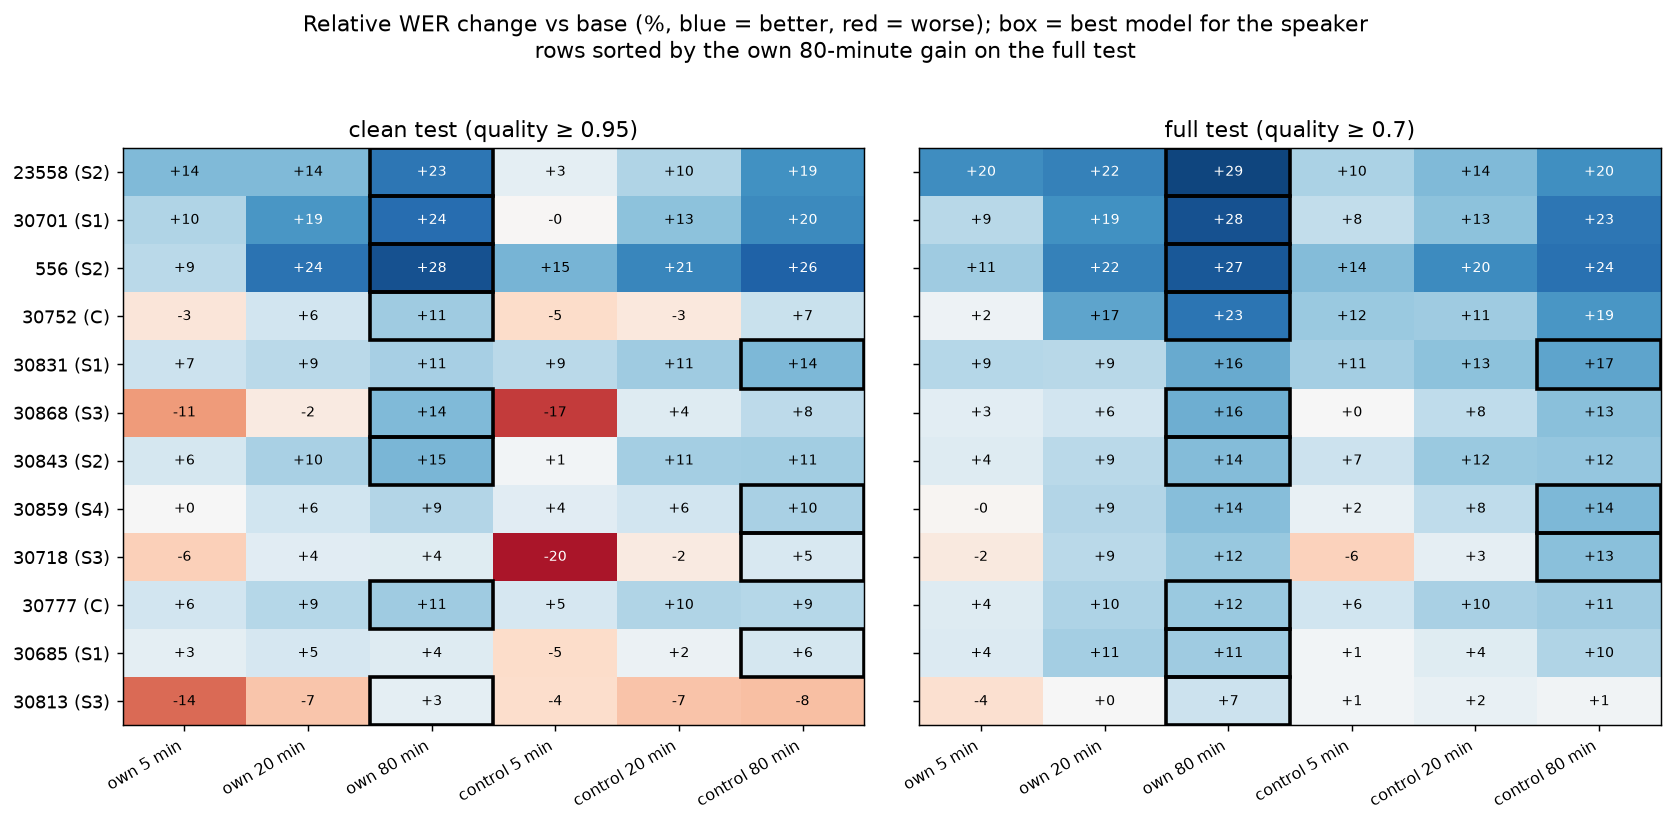
\includegraphics[width=0.9\textwidth]{figures/stage2_best_model_per_speaker.png}
    \caption{Relative WER change over arm~B (\%) for each speaker under each adapter;
    blue is better, red is worse, and the box marks the speaker's lowest WER. The
    80-minute columns are averaged over three seeds. Rows are sorted by the own
    80-minute gain on the full test.}
    \label{fig:bestmodel}
\end{figure*}

\paragraph{How Much Speaker Data Is Needed.}
The own adapter's median relative gain over arm~B grows from +4.3\% to +7.5\% to
+12.0\% on the clean test at 5, 20 and 80 minutes, and from +4.2\% to +9.7\% to
+15.3\% on the full test (Figure~\ref{fig:budget}); no 5- or 20-minute adapter is the
best model for any speaker (Figure~\ref{fig:bestmodel}). The control rises almost as
fast, to +0.3\%, +7.8\% and +10.1\% on the clean test and +6.7\%, +10.9\% and +14.3\%
on the full test, so what extra audio buys is mostly not specific to the speaker, and
the personal margin stays between +1.6\% and +3.1\% on the clean test at every
budget. At 5 minutes both adapters are unreliable: they are worse than arm~B for some
speakers, and the personal margin has opposite signs on the two test sets.

% TODO: add conclusions from the ongoing larger-data run (four speakers, well beyond
% 80 minutes each): does the gain, and the personal margin, keep growing with more
% speaker data?

\paragraph{Personal versus Shared Adaptation.}
At 80 minutes, the median personalization over the 36 speaker--seed pairs is +2.4\%
on the clean test and +2.2\% on the full test. With seed 0, the own adapter gains
+12.0\% and +15.3\%, while the control, which never heard the speaker, already gains
+10.1\% and +14.3\% (Figure~\ref{fig:budget}): most of the adaptation gain is general,
and the speaker's own audio adds 2--3\% on top of it.

Five speakers are significant in all three seeds on the full test
(Figure~\ref{fig:perspeaker}), led by 23558 at +9\% to +10\%; six never are, in any
seed or test. Profile does not predict the effect: speakers the fine-tune helped least
and speakers hard under both models fall on both sides. A speaker's personalization
varies across seeds with a median standard deviation of 2.4\% on the clean test, as
large as the effect, so we make per-speaker claims only where all seeds agree. Nor
does the margin grow on cleaner audio: by alignment-quality band of the full test,
own adapter and control gain alike on the two hardest bands (about +20\%), and the
median personalization is +0.5\%, +4.0\%, +2.5\% and +2.3\% from the hardest band to
the cleanest.

% Full width: 12 speakers x 3 seeds with intervals, on two test sets.
\begin{figure*}[t]
    \centering
    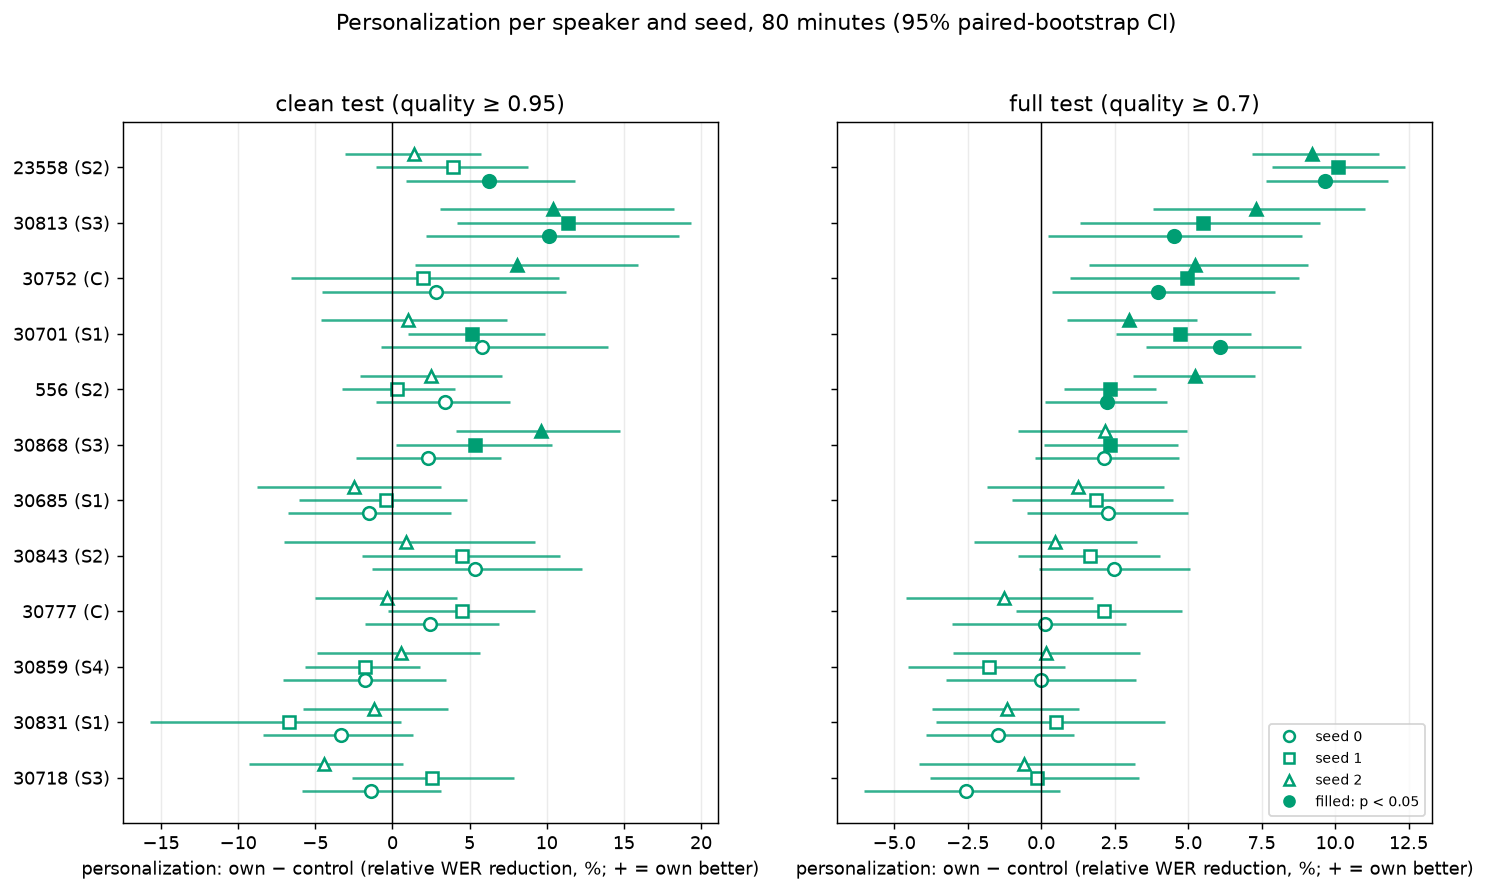
\includegraphics[width=0.85\textwidth]{figures/stage2_personalization_per_speaker_seeds.png}
    \caption{Personalization (own $-$ control, relative WER reduction in \%) per speaker
    and seed at 80 minutes, on the clean test (left) and the full test (right), with
    95\% paired-bootstrap intervals. Filled markers: own adapter significantly better
    than the control (paired bootstrap, $p<0.05$); hollow: not significant. Speakers are
    sorted by their mean on the full test. Profiles: S1, helped least by the fine-tune;
    S2, hard under both models; S3, typical; S4, low WER; C, high-gain control.}
    \label{fig:perspeaker}
\end{figure*}

\paragraph{Learning Curves.}
Validation loss reaches its minimum at step 60--100, about two passes over the data
and 38--54\% below the validation loss of arm~B without an adapter, and then rises as
the adapter overfits (Figure~\ref{fig:lc}). Every run stops early, by step 180 of 400,
and the three seeds trace nearly identical curves (Figure~\ref{fig:lcspeakers},
Appendix~\ref{app:additional}). An adapter trains in under two minutes on one GPU.

\begin{figure}[t]
    \centering
    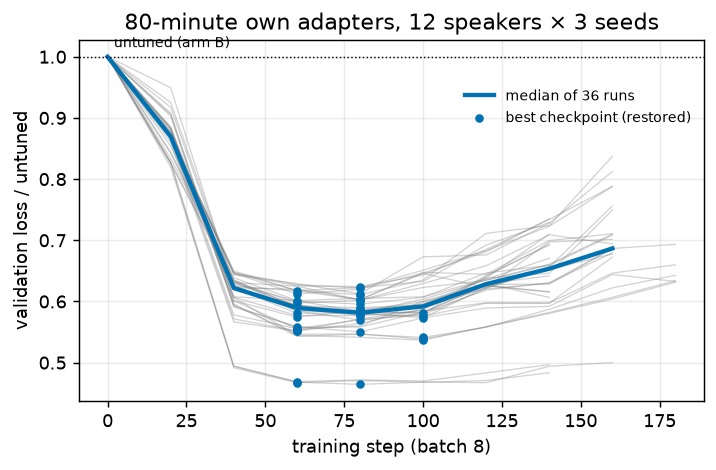
\includegraphics[width=\columnwidth]{figures/stage2_winning_learning_curves_compact.png}
    \caption{Validation loss relative to arm~B while training the 80-minute own adapters
    (12 speakers $\times$ 3 seeds). Thin lines: one run each; thick: the median; dots:
    the checkpoints early stopping restored.}
    \label{fig:lc}
\end{figure}


% ============================================================
% CONCLUSION
% ============================================================

\section{Conclusion}

The Hebrew fine-tune lowers every speaker's error but leaves them as unequal as
before, which motivates adapting to individual speakers.

\paragraph{Most of the adaptation gain is general.}
An 80-minute LoRA adapter on a speaker's own committee speech lowers arm~B's WER by a
median 12\% on the clean test and 15\% on the full test; the same amount of other
speakers' audio already lowers it by 10\% and 14\%. Training on the speaker's own
audio adds a further 2--3\% over this shared baseline, an effect that is stable
across seeds.

\paragraph{More audio gives more gain, but mostly not personal gain.}
From 5 to 80 minutes the own adapter's gain roughly triples, and the control's grows
almost as fast.

\paragraph{Adaptation is cheap.}
An adapter converges in about two passes over its data. The recipe is insensitive to
rank, augmentation and, at 80 minutes, the learning rate, but Whisper's dropout
prevents learning.

Whether the personal margin grows with substantially more speaker data is tested in a
follow-up on four speakers, now running. Further directions are adaptation on similar
rather than random speakers and evaluation against verbatim human transcripts.


% ============================================================
% LIMITATIONS
% ============================================================

\section*{Limitations}

\paragraph{Prior exposure.} Arm~B was fine-tuned on Knesset plenary speech, which
includes many of our speakers. Our evaluation uses committee recordings, a different setting and register, but the model may still be partly familiar with these voices.

\paragraph{Shared recording conditions.} Train and test sets are meeting-disjoint,
but not committee-disjoint: about 75--82\% of the test speech comes from committees the same speaker also appears in during training, and so likely from the same rooms and microphones. Part of an adapter's gain may therefore reflect familiar recording conditions rather than the voice alone.

\paragraph{The reference is the protocol.} Every WER is measured against the
stenographic protocol, which is not a verbatim transcript. Our gains are gains in
agreement with the protocol, and may partly reflect learning what the stenographer
omits. We limit this by training and validating only on segments whose protocol
closely matches the audio (quality $\geq 0.95$, Appendix~\ref{app:data}). That score,
however, comes from a Whisper-family aligner, so a test set filtered the same way would
favour speech that Whisper models already transcribe well; we therefore score every
model both on the high-quality segments and on all segments at quality $\geq 0.7$.
Whether the personal margin is larger against what was actually said requires a human
verbatim reference.

% TODO (decide later): "The reference is the protocol" (Hadas) and "Reference
% transcripts" (Dolev) cover the same limitation. Both are kept for now. Keep one,
% or fold the ivrit.ai consultation point into the other.
\paragraph{Reference transcripts.} Our references are the Knesset's stenographic
protocols, not verbatim transcripts: stenographers condense, rephrase and omit
speech, so part of every measured error is a mismatch between protocol and audio
rather than a recognition mistake. We limit this with alignment-quality filters set
in consultation with the ivrit.ai team (Section~\ref{sec:preprocessing},
Appendix~\ref{app:data}), but no verbatim, human-transcribed test set was available.
Absolute WERs therefore partly reflect the protocol's editing, and our comparisons
are most reliable between models scored against the same references.

\paragraph{Limited compute.} Training and inference ran on paid cloud services
(RunPod GPUs and Hugging Face inference), at a total cost of about \$200 across all
our experiments. Within this budget we focused on the experiments central to our
question, and a larger budget would allow more models, configurations and speakers
to be explored.

\paragraph{Tuning on validation loss.} The rank, dropout, augmentation and learning
rate were chosen on the validation loss of four speakers. The rejected settings,
including rank 16, were never scored on the test sets.

\paragraph{A random control group.} The control pools speakers at random, so it does
not test whether \emph{similar} speakers could replace a speaker's own audio; we leave
that comparison to future work.


% ============================================================
% ACKNOWLEDGMENTS
% ============================================================

\section*{Acknowledgments}

We thank the ivrit.ai team (\href{https://www.ivrit.ai}{ivrit.ai}, with models and
datasets at \url{https://huggingface.co/ivrit-ai}, and \citealp{marmor2025hebrewasr})
for their support throughout this project. Their openness in sharing ideas,
practical advice and lessons from their own work on Hebrew speech data helped shape
our direction, and their open models and datasets made this study possible.


% ============================================================
% REFERENCES
% ============================================================

% This assumes your bibliography file is named custom.bib.
\bibliography{custom}


% ============================================================
% APPENDICES
% ============================================================

\appendix


% ------------------------------------------------------------
\section{Data Preparation Details}
\label{app:data}

\paragraph{Alignment quality score.}
The corpus aligns each protocol to its recording with a Whisper-family forced aligner,
which assigns every protocol word a time span and a probability: how likely the model
finds that word at that point in the audio. A protocol segment's quality score is the
median probability of its words. Our segments of up to 30 seconds can join several
protocol segments, so their score is the duration-weighted median over those parts.
A low score means the text and the audio disagree, potentially because the stenographer
condensed or omitted speech, or because of cross-talk. ivrit.ai treat 0.65 as fit for
training and 0.95 as high quality.

\paragraph{Quality filter for the analysis.}
The 0.7 threshold removes 7{,}810 of 65{,}990 segments (11.8\%, 12.8 hours). Removing them lowers the corpus WER
from 0.417 to 0.387 (A) and from 0.324 to 0.292 (B), and leaves the difference between
the arms almost unchanged.

\paragraph{Quality filter for training.}
Because the score is a median, a segment can pass it while a few of its words are misaligned. Training and validation segments therefore use the word
probabilities directly and must pass four conditions: confidence at least 0.95, at
most 10\% of words with probability below 0.5, no run of three or more such words,
and the number of aligned words falling within the segment's time span matches the
number of words in its reference text to within 20\%, so that the word probabilities
checked above actually cover the segment's text.

\paragraph{Two test sets.}
The aligner is itself a Whisper-family model, so a 0.95 threshold favours segments that
Whisper models already transcribe well. Applied to the test set, this introduces a
selection bias toward easy speech. We therefore score every
model on two test sets drawn from the same held-out sessions: the filtered segments, and
all segments with confidence of at least 0.7.

% ------------------------------------------------------------
\section{Training Details}
\label{app:training}

All settings were chosen on validation loss alone, in 64 tuning runs that never
touched the test sets; the result is Table~\ref{tab:hyperparams}, shared by every own
and control adapter.

\paragraph{Tuning procedure.}
Four tuning speakers, one per profile (30685, S1; 23558, S2; 30718, S3; 30859, S4),
were trained at the two ends of the budget range, 5 and 80 minutes; 20 minutes takes
the 80-minute choice. The criterion is the relative drop in validation loss from arm~B
to the best checkpoint. Tuning ran in three stages, each starting from the previous
stage's choice: the learning rate ($10^{-4}$, $3\times10^{-4}$, $10^{-3}$); LoRA rank
$\{8, 16\}$ $\times$ Whisper's dropout $\{0, 0.1\}$; and augmentation (SpecAugment,
alone or with $\pm10\%$ tempo changes; no pitch or speed perturbation, which would
change the voice). A setting replaces the simpler incumbent ($3\times10^{-4}$, rank 8,
no dropout, no augmentation) only if it raises the mean drop by at least 0.01 and helps
at least three of the four speakers.

\paragraph{Tuning results} (Figures~\ref{fig:tuningscores} and~\ref{fig:tuningcurves}).
\begin{itemize}
    \item \textbf{Learning rate matters only at 5 minutes.} There, $10^{-4}$ gives a mean
    drop of 0.294 against 0.266 and 0.269 for the higher rates, whose best checkpoint
    comes at step 20--40, after which their validation loss rises above arm~B's. At 80
    minutes the three rates give 0.434, 0.432 and 0.429: early stopping absorbs the
    difference, so the incumbent $3\times10^{-4}$ stays.
    \item \textbf{Rank 16 adds nothing:} 0.432 at 80 minutes, equal to rank 8, and 0.281
    against 0.294 at 5 minutes.
    \item \textbf{Whisper's dropout prevents learning.} At 0.1, the drop collapses to
    0.019 at 5 minutes and 0.077 at 80 for every speaker.
    \item \textbf{Augmentation is within noise:} 0.298 and 0.300 at 5 minutes (below the
    0.01 threshold), 0.430 and 0.431 at 80.
\end{itemize}

\begin{table}[h]
\centering
\small
\begin{tabular}{lp{4.3cm}}
\toprule
Hyperparameter & Value \\
\midrule
Base model & \texttt{ivrit-ai/whisper-large-v3}, frozen, bfloat16 \\
Adapter & LoRA on the query and value projections of every attention layer (encoder, decoder self- and cross-attention) \\
Rank / $\alpha$ / LoRA dropout & 8 / 16 / 0.05 \\
Trainable parameters & 3{,}932{,}160 \\
Learning rate & $10^{-4}$ at 5 minutes; $3\times10^{-4}$ at 20 and 80 minutes \\
Schedule & constant after 20 warm-up steps \\
Batch size & 8, no gradient accumulation \\
Weight decay & 0.01 \\
Whisper dropout & 0 \\
Augmentation & none \\
Training length & at most 400 steps \\
Validation & loss every 20 steps \\
Early stopping & after 4 validations without improvement; best checkpoint restored \\
Training labels & protocol text \\
Seeds & 0 at every budget; 1 and 2 at 80 minutes \\
\bottomrule
\end{tabular}
\caption{Training hyperparameters, identical for every own and control adapter.}
\label{tab:hyperparams}
\end{table}

\begin{figure*}[t]
    \centering
    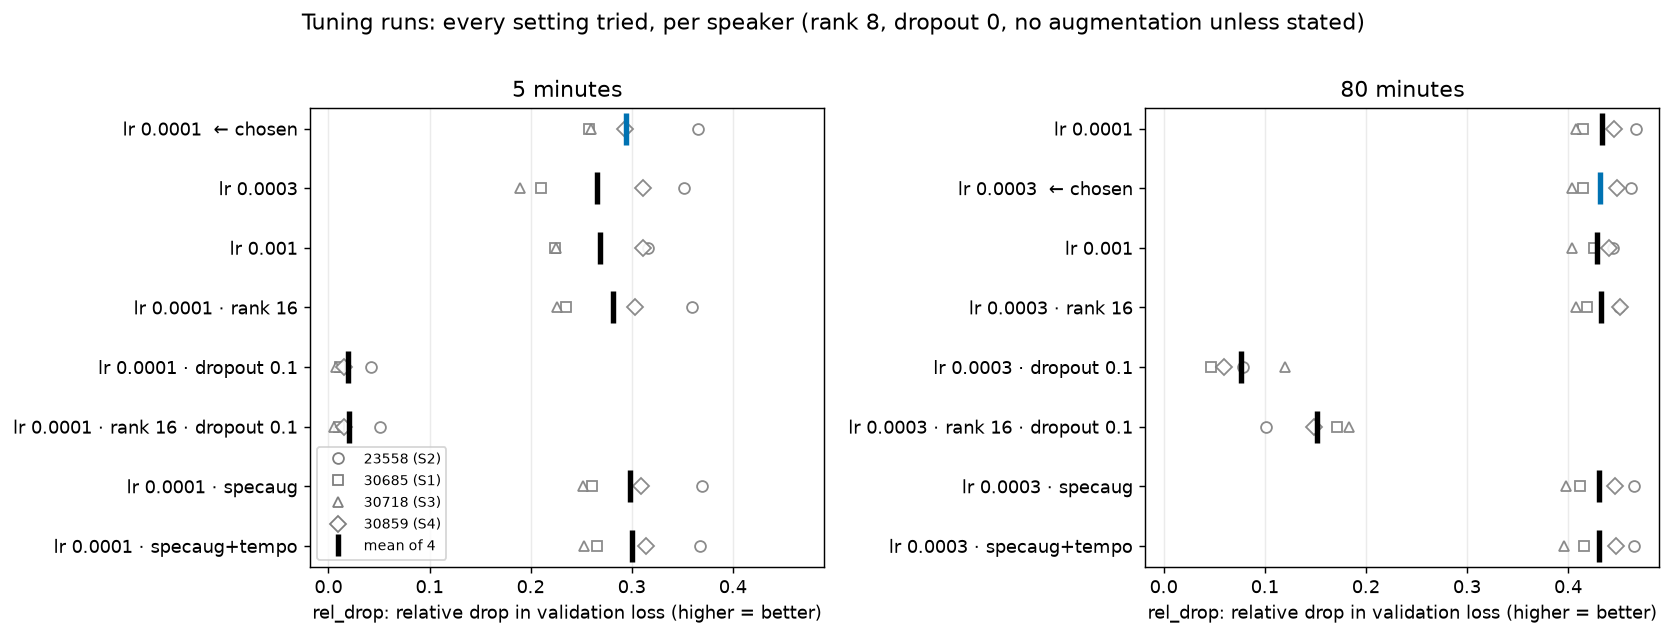
\includegraphics[width=\textwidth]{figures/stage2_tuning_scores.png}
    \caption{Every tuning run, at 5 minutes (left) and 80 minutes (right). Markers: the
    four tuning speakers; bar: their mean; blue: the chosen setting. The x-axis is the
    relative drop in validation loss from arm~B to the best checkpoint.}
    \label{fig:tuningscores}
\end{figure*}

\begin{figure*}[t]
    \centering
    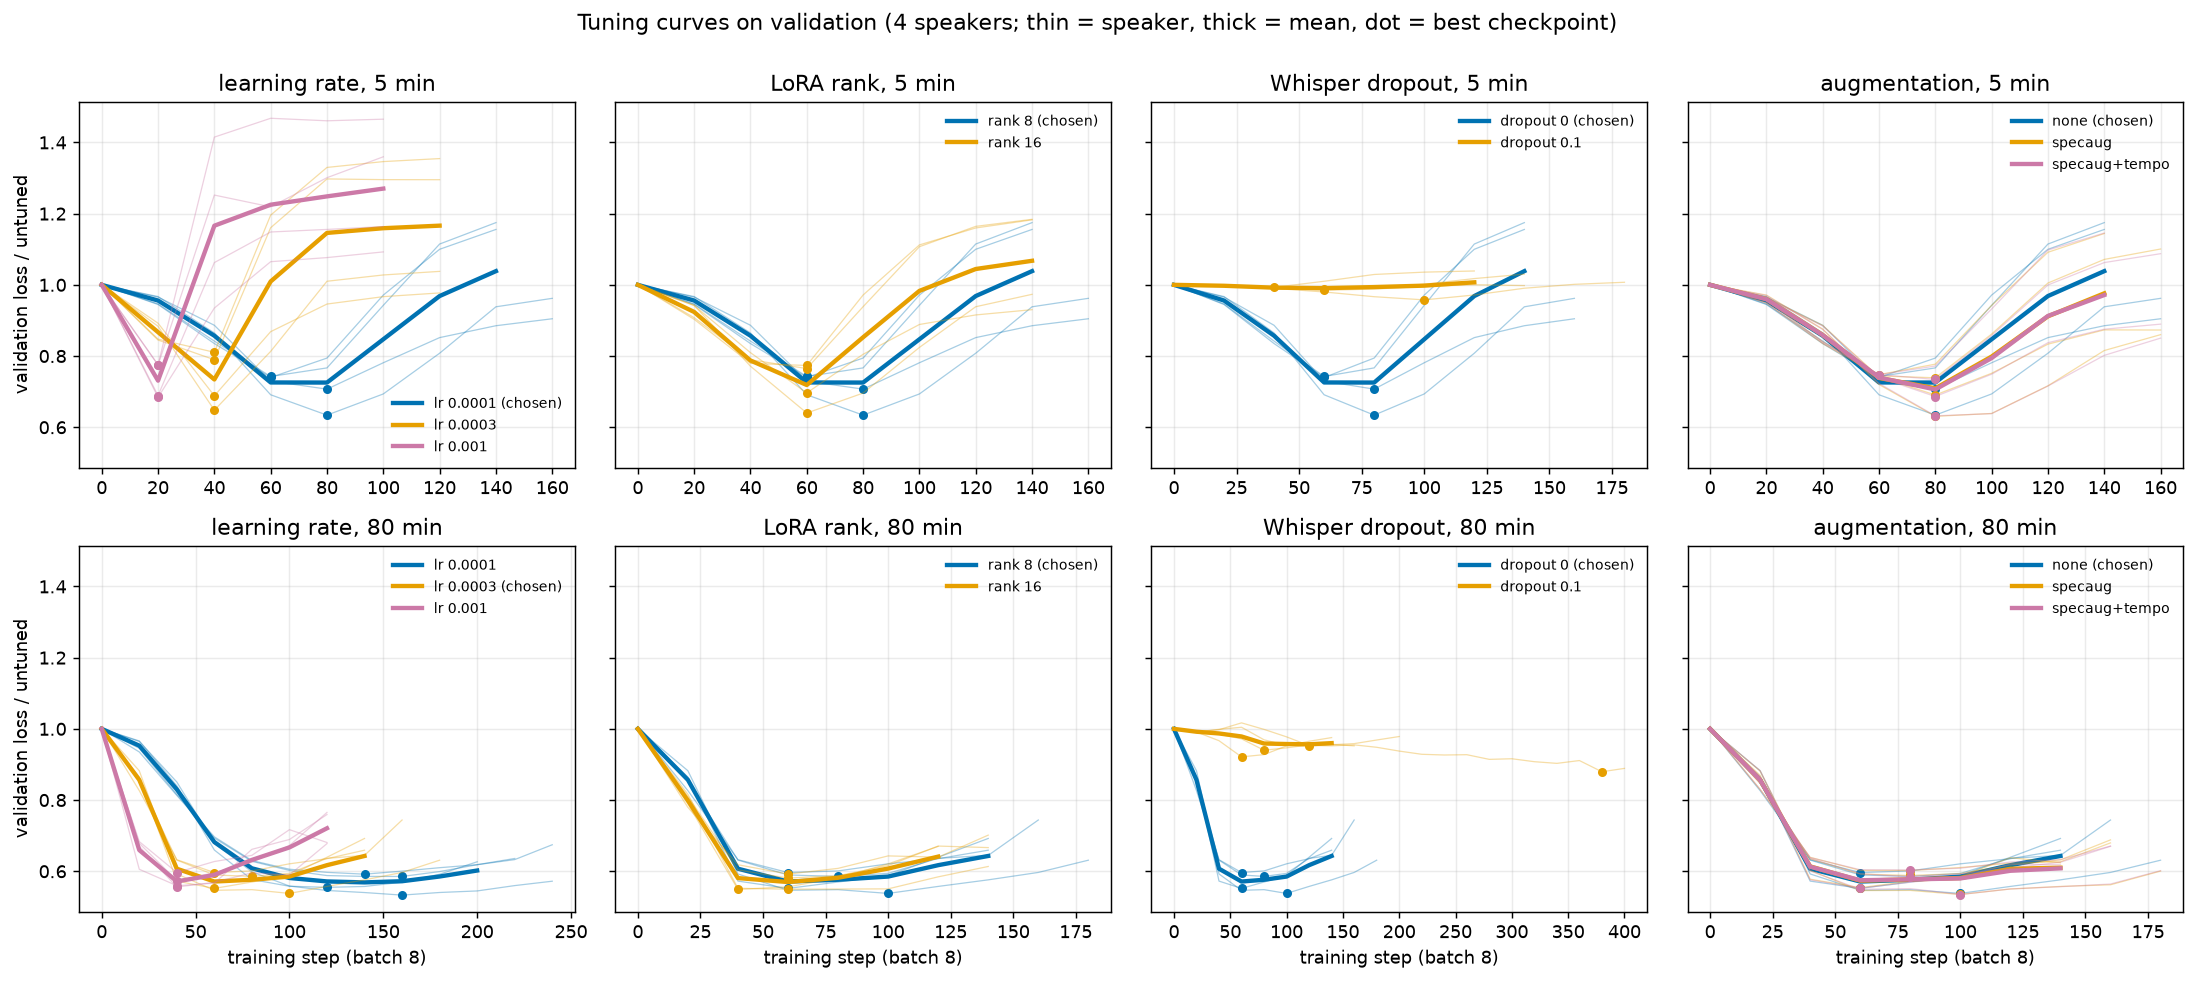
\includegraphics[width=\textwidth]{figures/stage2_tuning_curves.png}
    \caption{Validation loss relative to arm~B during tuning, varying one setting at a
    time around the chosen recipe, at 5 minutes (top) and 80 minutes (bottom). Thin
    lines: the four speakers; thick: their mean; dots: the best checkpoints.}
    \label{fig:tuningcurves}
\end{figure*}


% ------------------------------------------------------------
\section{Implementation Details}
\label{app:implementation}

\paragraph{Training.}
Adapters are trained with PyTorch, Hugging Face \texttt{transformers}
(\texttt{Seq2SeqTrainer}) and \texttt{peft}, on the frozen base model in bfloat16.
Training segments are fed latest meeting first, so the 5-, 20- and 80-minute budgets
are nested prefixes of one ordering. Each control's pool takes one segment from each
of its six speakers in turn until the budget is reached.

\paragraph{Scoring.}
Reference and hypothesis are normalized (niqqud and punctuation removed) and aligned
word by word; substitutions, deletions and insertions are counted per segment. WER is
pooled over a speaker's test set: the sum of word errors divided by the sum of
reference words. Confidence intervals and p-values come from a paired bootstrap over
test segments (2{,}000 resamples, two-sided p); for personalization, the own and
control hypotheses of the same segments are resampled together.


% ------------------------------------------------------------
\section{Additional Results}
\label{app:additional}

\subsection{Speaker-Level Error Map}

\begin{figure}[h]
    \centering
    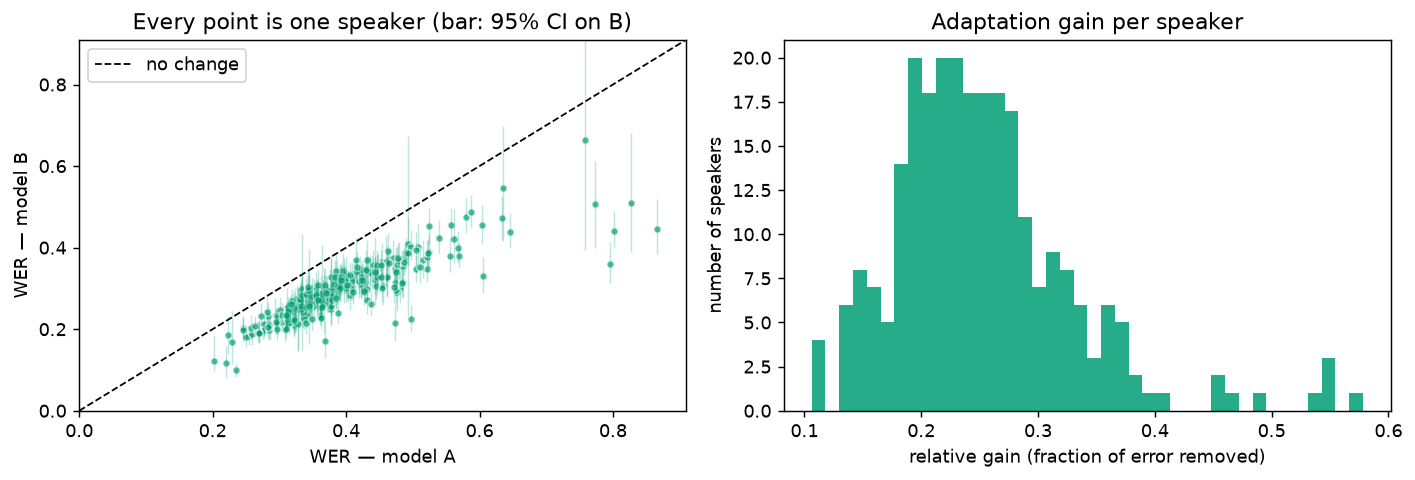
\includegraphics[width=\columnwidth]{figures/error_map_gain.png}
    \caption{Left: per-speaker WER under arm~A against arm~B. Every point is one
    speaker, the bar is the 95\% bootstrap interval on WER$_B$ and the dashed line is
    no change. Right: distribution of the relative gain over the 261 speakers with at
    least 20 segments.}
    \label{fig:gain}
\end{figure}

\paragraph{Reliability of the per-speaker measures.}
Each speaker is measured on about one hour of speech, so their WER and gain carry
sampling noise. To test whether the differences between speakers are a stable property
of the speakers rather than of the particular sample, we split each speaker's sessions
into two alternating halves, compute WER$_B$ and the relative gain on each half
independently, and compare the halves across speakers (Figure~\ref{fig:reliability}).
If the differences were noise, the two halves would be unrelated and the points would
form a shapeless cloud. If they are stable, the points follow the diagonal. They do:
the correlation between halves, corrected to full length (Spearman--Brown), gives a
reliability of 0.78 for WER$_B$ and 0.75 for relative gain. This is what
justifies ranking speakers by their gain when selecting them for personalization.

\begin{figure}[h]
    \centering
    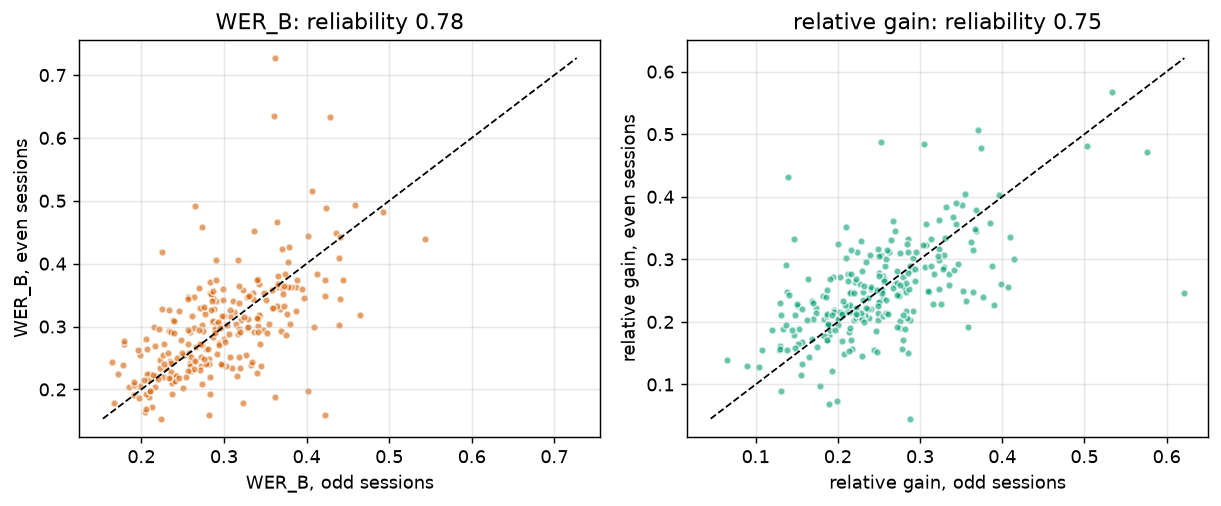
\includegraphics[width=\columnwidth]{figures/error_map_reliability.png}
    \caption{Each point is one speaker, measured separately on their odd and even
    sessions. Points near the diagonal mean the measure repeats across recordings,
    and titles give the split-half reliability (Spearman--Brown corrected).}
    \label{fig:reliability}
\end{figure}

\paragraph{Gain by group.}
Figure~\ref{fig:groups} shows the gain for the six groupings not shown in the main text
(speaking rate is Figure~\ref{fig:rate}). Speakers with missing metadata and groups of
fewer than three speakers are omitted.

\begin{figure*}[t]
    \centering
    \begin{subfigure}[b]{0.49\textwidth}
        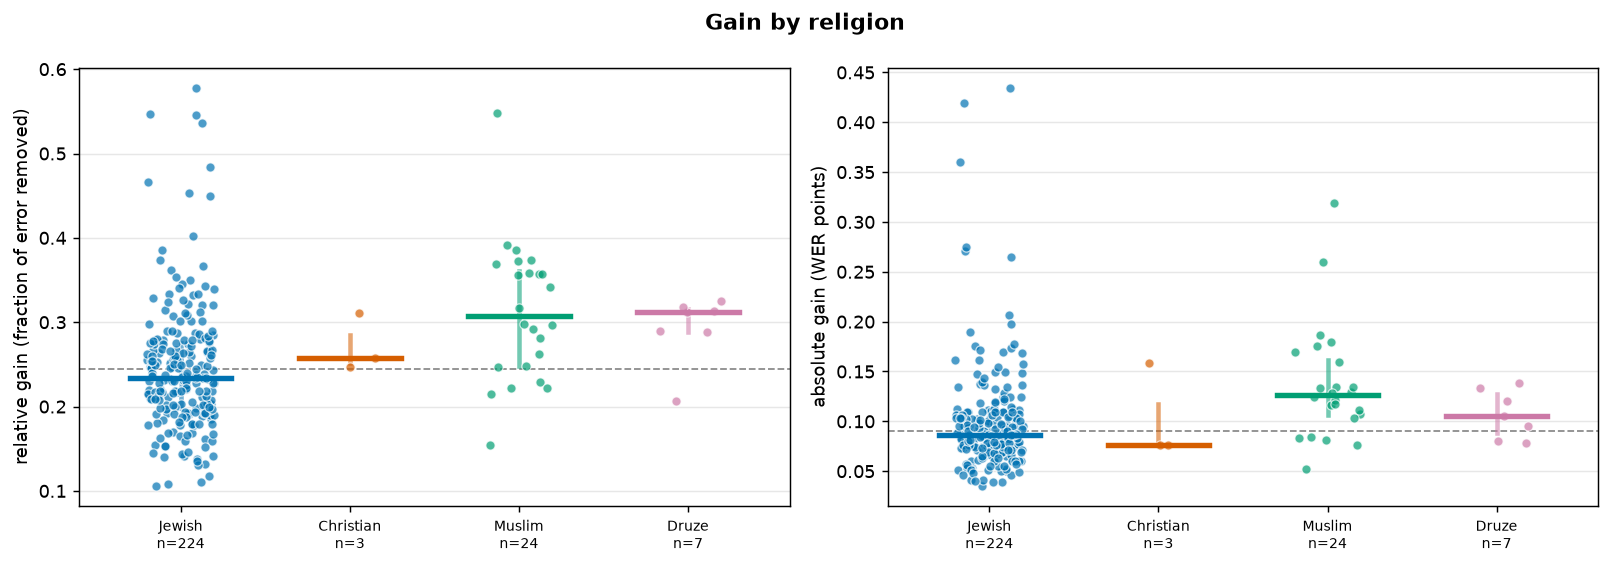
\includegraphics[width=\linewidth]{figures/group_religion.png}
        \caption{Religion}
    \end{subfigure}\hfill
    \begin{subfigure}[b]{0.49\textwidth}
        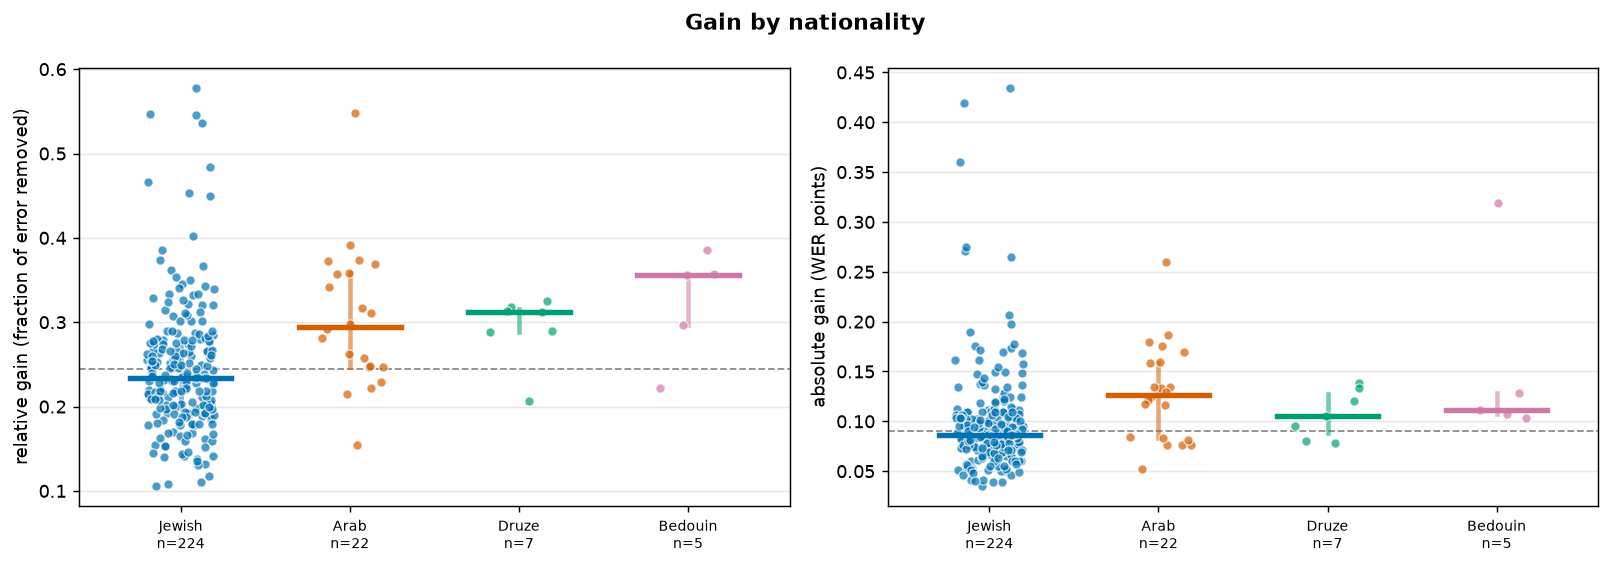
\includegraphics[width=\linewidth]{figures/group_nationality.png}
        \caption{Nationality}
    \end{subfigure}
    \par\medskip
    \begin{subfigure}[b]{0.49\textwidth}
        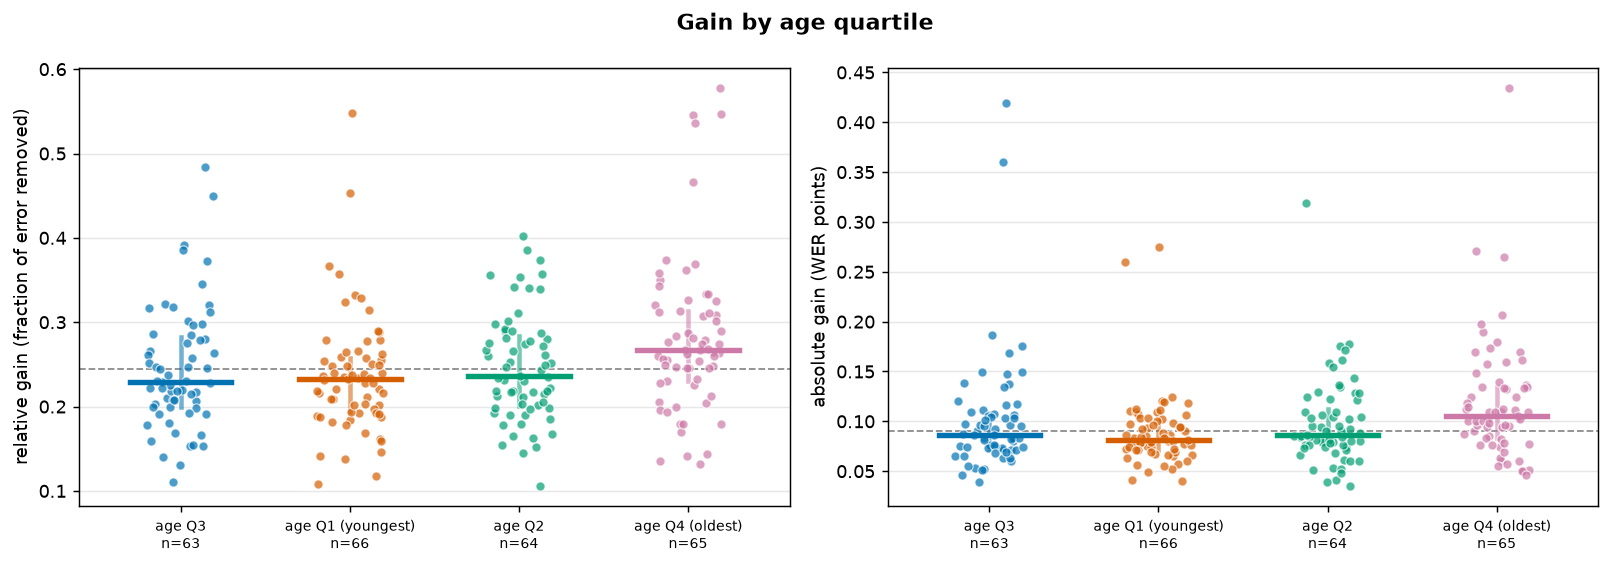
\includegraphics[width=\linewidth]{figures/group_age_band.png}
        \caption{Age quartile}
    \end{subfigure}\hfill
    \begin{subfigure}[b]{0.49\textwidth}
        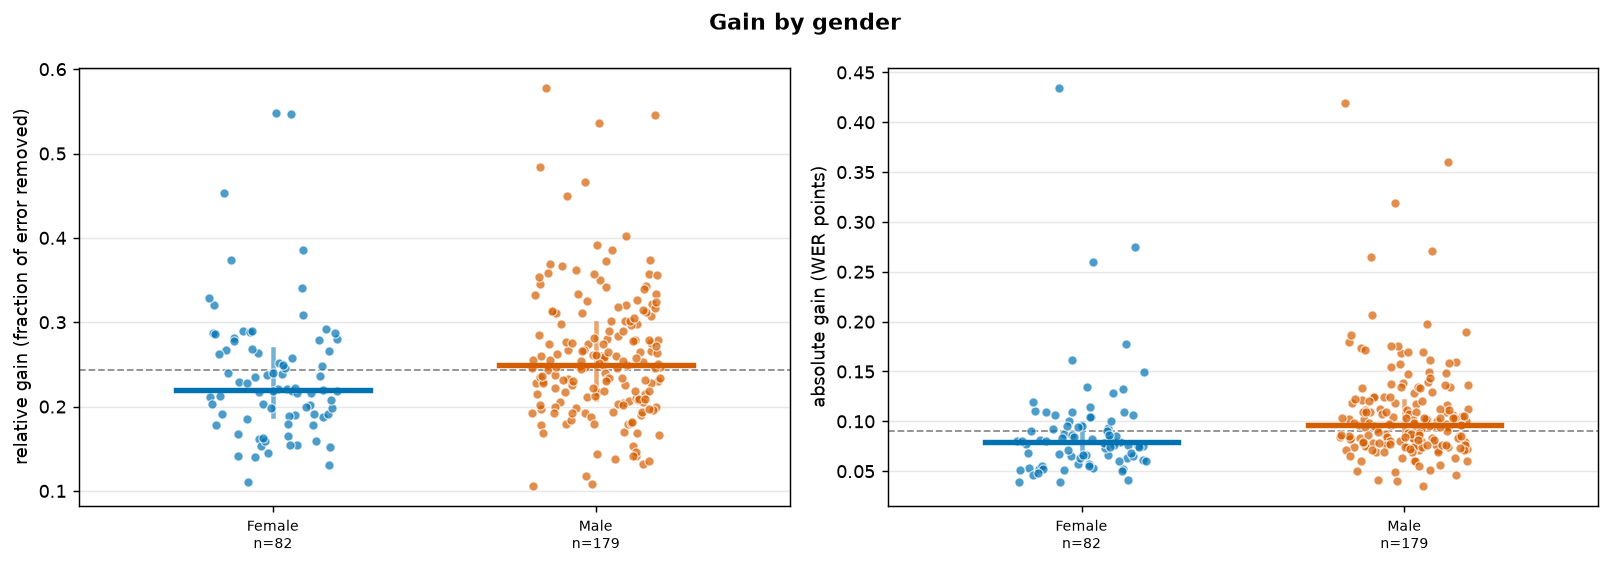
\includegraphics[width=\linewidth]{figures/group_gender.png}
        \caption{Gender}
    \end{subfigure}
    \par\medskip
    \begin{subfigure}[b]{0.49\textwidth}
        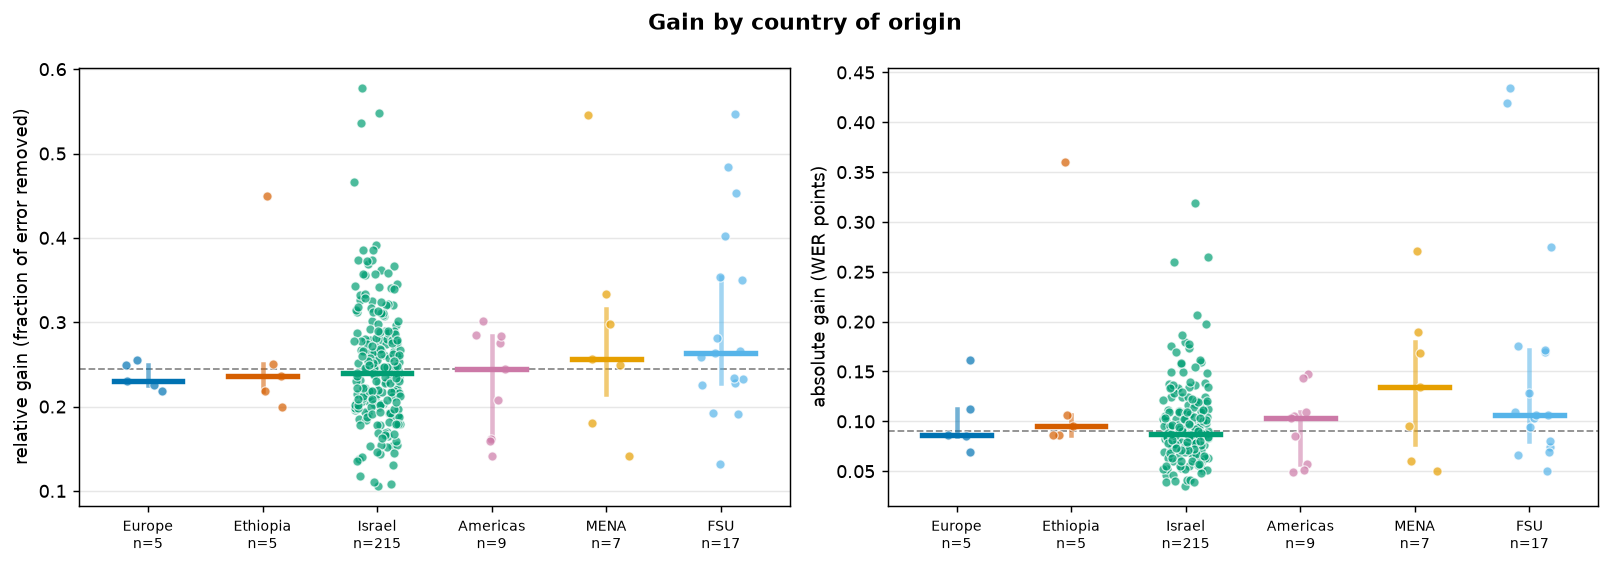
\includegraphics[width=\linewidth]{figures/group_origin.png}
        \caption{Country of origin}
    \end{subfigure}\hfill
    \begin{subfigure}[b]{0.49\textwidth}
        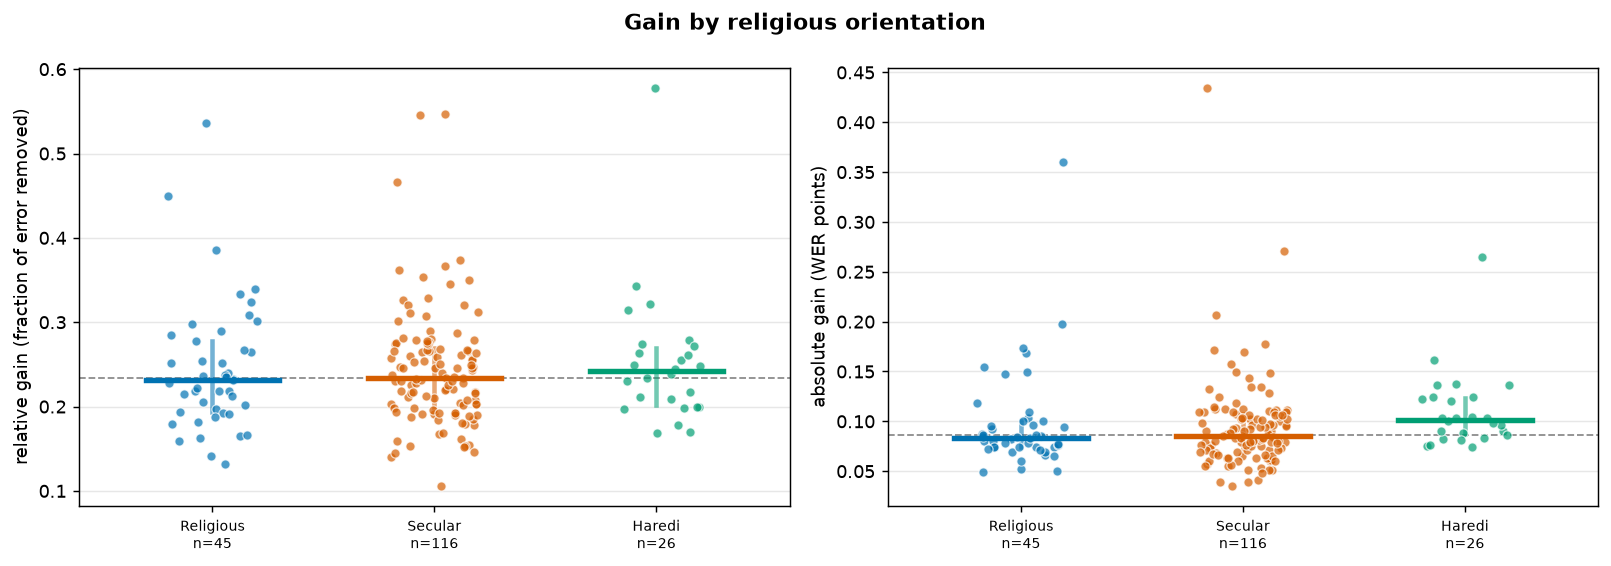
\includegraphics[width=\linewidth]{figures/group_orientation.png}
        \caption{Religious orientation}
    \end{subfigure}
    \caption{Gain from the Hebrew fine-tune by group, relative (left of each panel) and
    absolute (right). Each point is one speaker with at least 20 segments. The bar is the
    group median, the line the interquartile range, and the dashed line the overall
    median.}
    \label{fig:groups}
\end{figure*}

\paragraph{Protocol omissions.}
Over half of arm~B's errors are insertions (Table~\ref{tab:errormix}), and 73\% of
its inserted words also appear in arm~A's transcript of the same segment. Agreement
between the two models does not show that a word was spoken: on a sample of
human-corrected clips, only about half of such words (19 of 36) were. Part of
arm~B's insertion errors therefore reflects speech the stenographic protocol left
out, and part reflects genuine recognition errors. All WERs in this paper are
computed against the protocol as is.

\begin{table}[h]
\centering
\small
\begin{tabular}{lccccc}
\toprule
& & & \multicolumn{3}{c}{share of word errors} \\
\cmidrule(lr){4-6}
Model & WER & CER & Sub. & Del. & Ins. \\
\midrule
A (general) & 0.387 & 0.241 & 49\% & 13\% & 38\% \\
B (Hebrew fine-tune) & 0.292 & 0.203 & 36\% & 11\% & 53\% \\
\bottomrule
\end{tabular}
\caption{Corpus error rates after the quality filter (267 speakers, 58{,}180 segments)
and the composition of each model's word errors: substitutions, deletions and
insertions.}
\label{tab:errormix}
\end{table}

\paragraph{Recording conditions.}
WER also varies with the recording conditions: arm~B scores 0.32--0.37 in 2018--2019
and 0.27--0.29 from 2020 on (Figure~\ref{fig:year}), and 0.21--0.37 across the twelve
largest committees.
Personalization splits are therefore meeting-disjoint and ordered by date: each speaker
is adapted on earlier meetings and tested on their newest ones, which is also how a personalized model would be used in practice.

\begin{figure}[h]
    \centering
    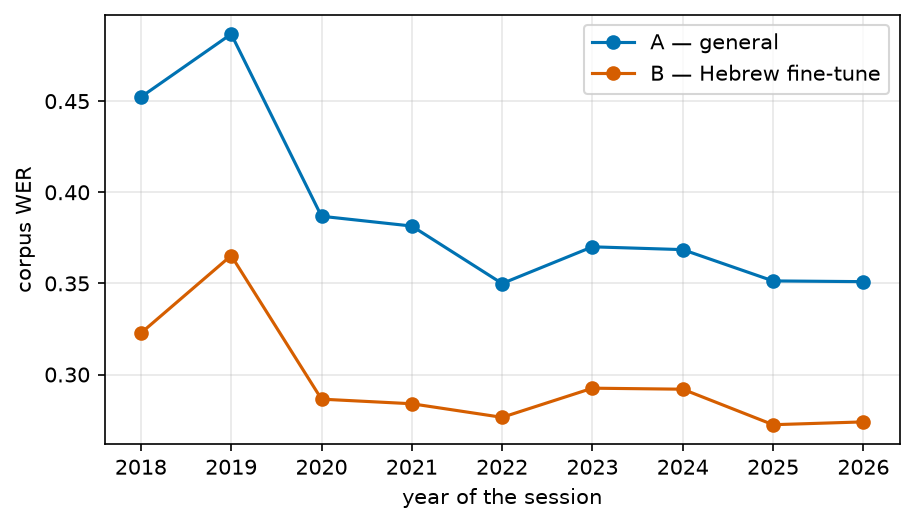
\includegraphics[width=\columnwidth]{figures/conditions_by_year.png}
    \caption{Corpus WER of both models by the year of the session, after the quality
    filter.}
    \label{fig:year}
\end{figure}

\subsection{Personalization}

\begin{figure}[h]
    \centering
    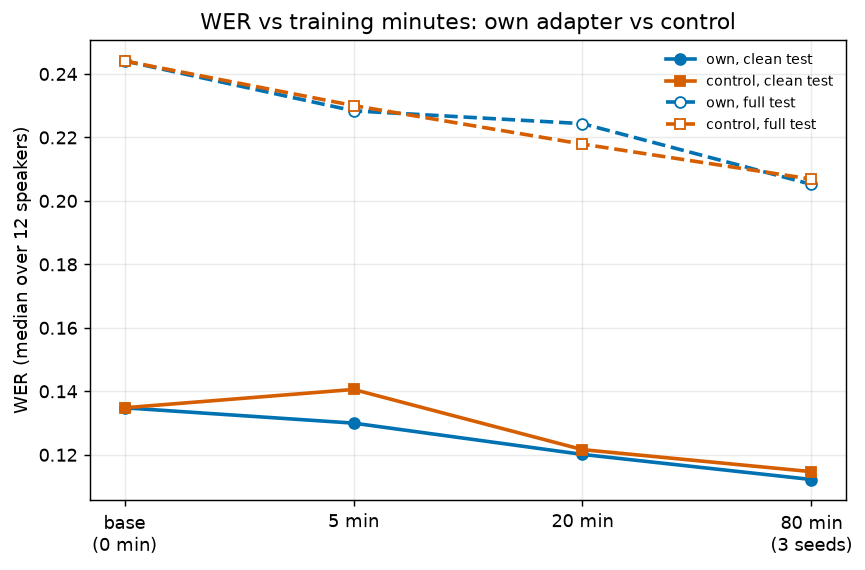
\includegraphics[width=\columnwidth]{figures/stage2_wer_vs_minutes_median.png}
    \caption{Median WER over the 12 speakers at 0 (arm~B), 5, 20 and 80 minutes of
    training audio, for the own adapter (blue) and the control (orange), on the clean
    test (solid) and the full test (dashed). At 80 minutes, each speaker's WER is
    averaged over three seeds.}
    \label{fig:wermedian}
\end{figure}

\begin{figure*}[t]
    \centering
    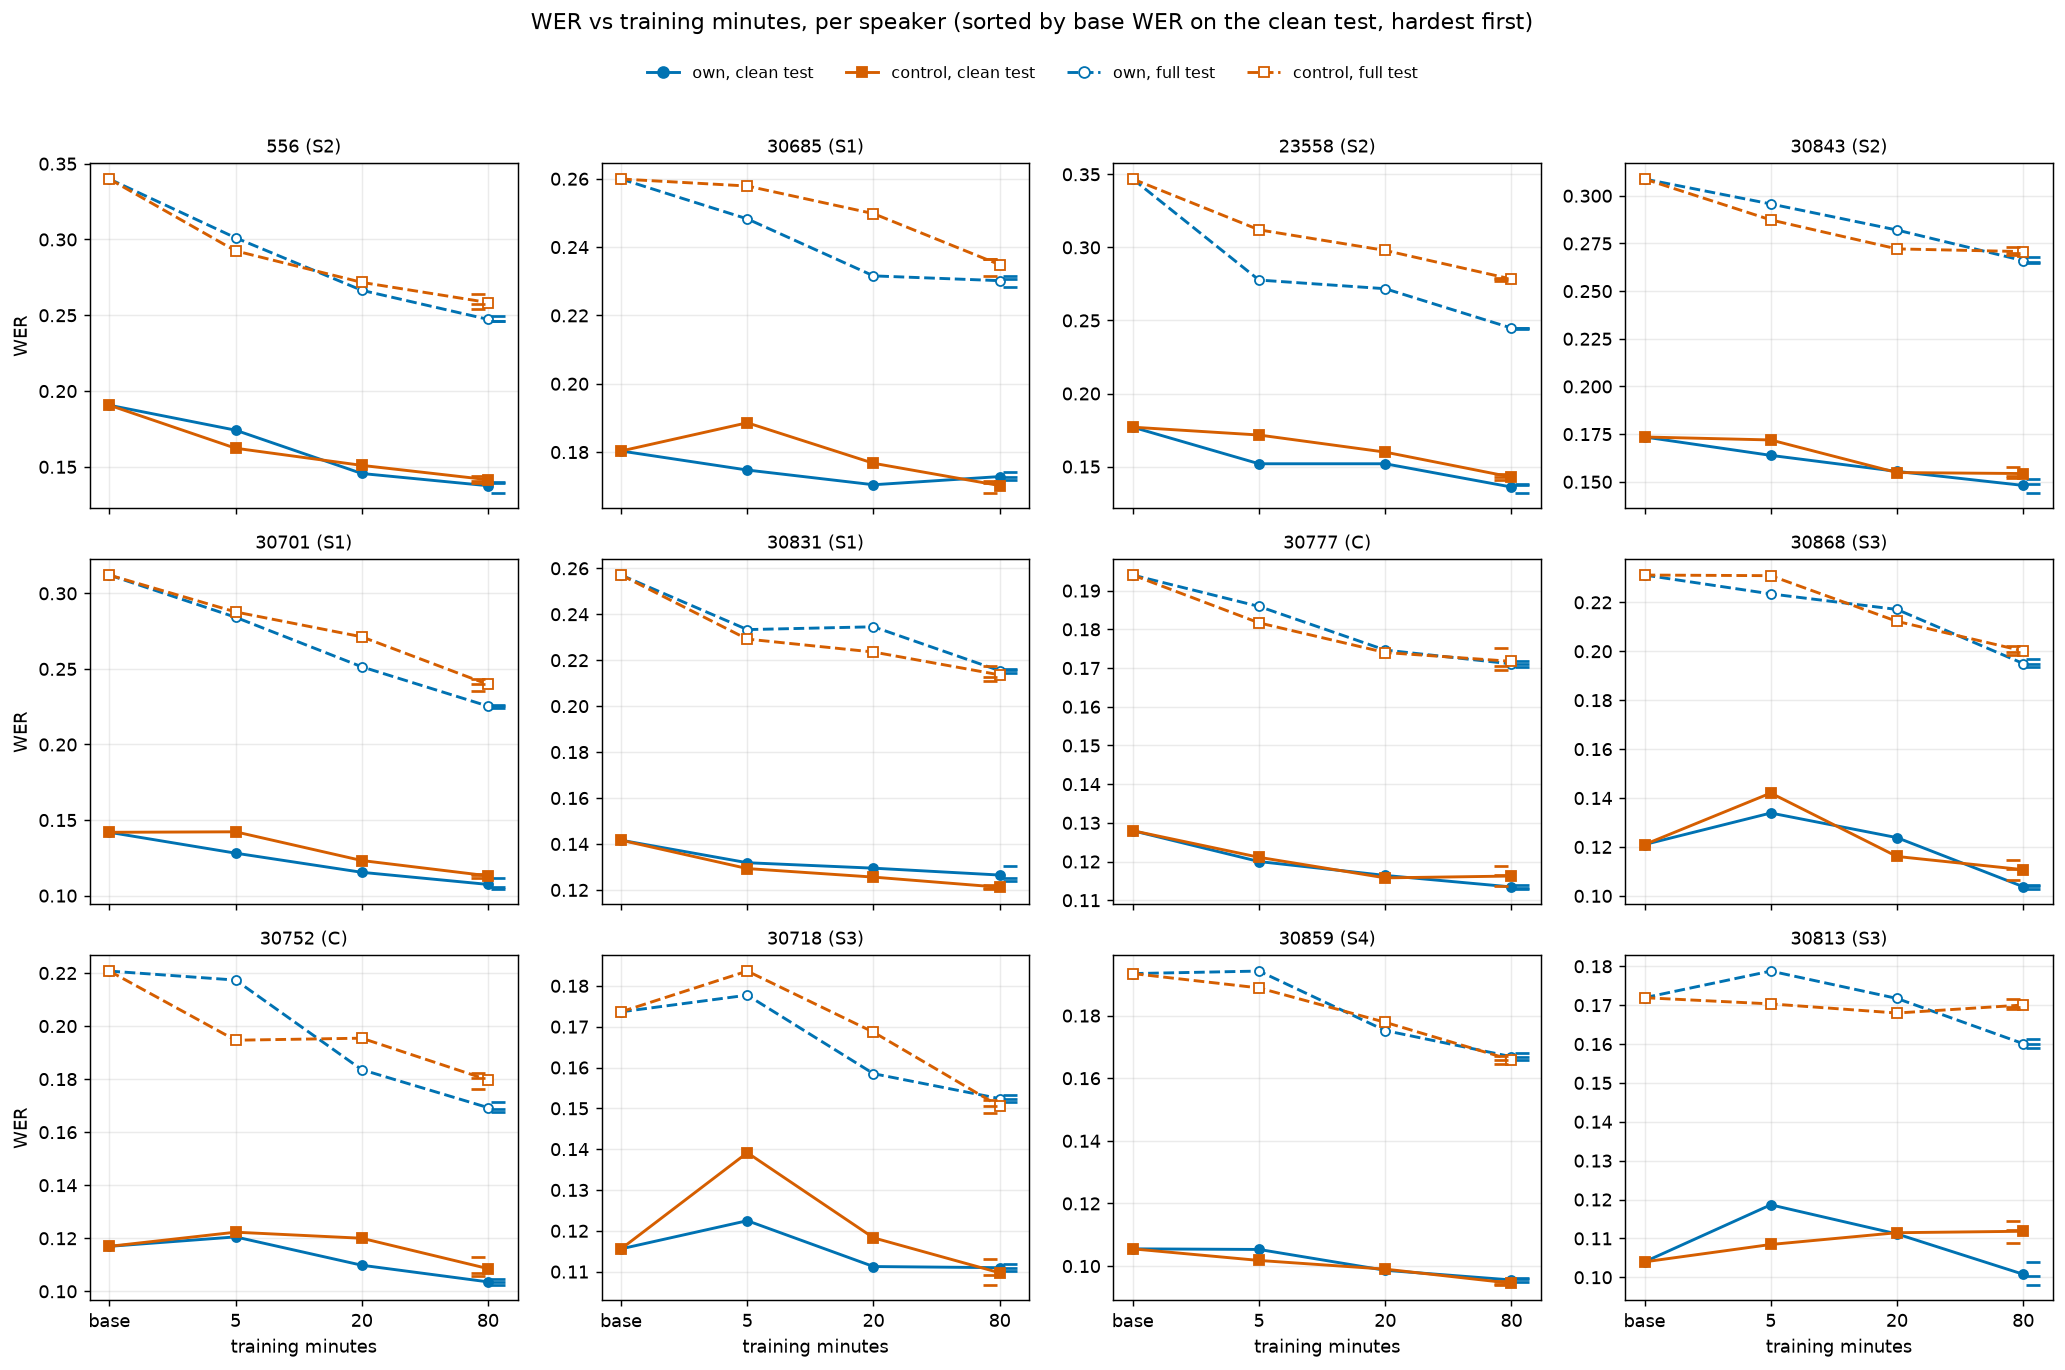
\includegraphics[width=\textwidth]{figures/stage2_wer_vs_minutes_per_speaker.png}
    \caption{The same per speaker, sorted by arm~B's WER on the clean test, hardest
    first. Ticks at 80 minutes: the individual seeds.}
    \label{fig:werspeaker}
\end{figure*}

\begin{figure*}[t]
    \centering
    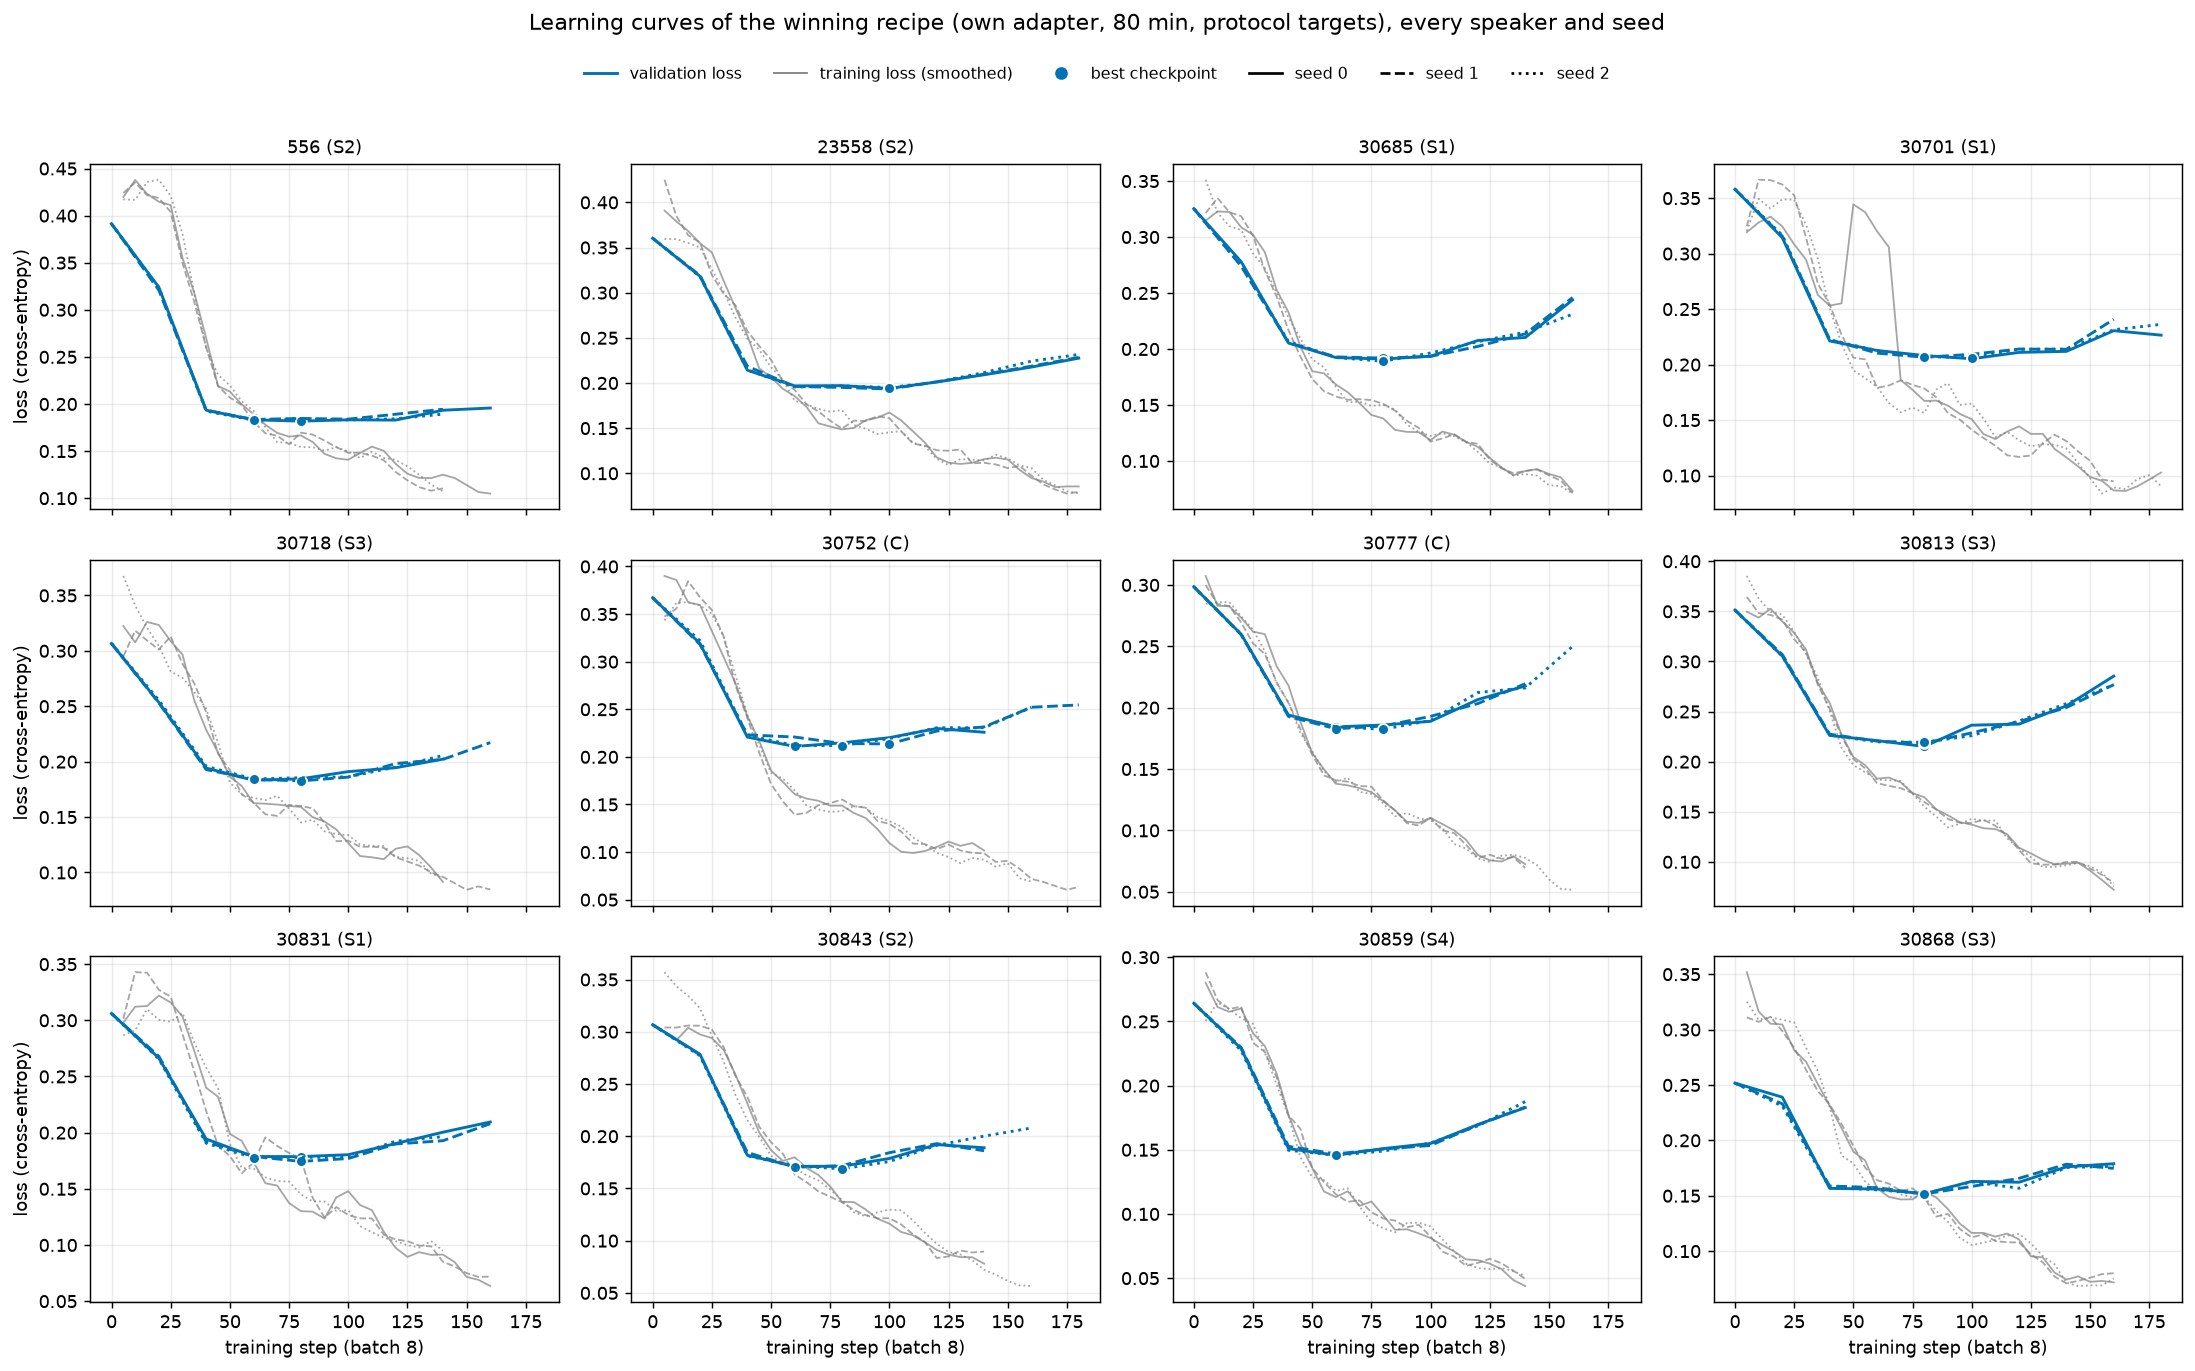
\includegraphics[width=\textwidth]{figures/stage2_winning_learning_curves.png}
    \caption{Learning curves of the 80-minute own adapters, one panel per speaker. Blue:
    validation loss every 20 steps (step 0 is arm~B); grey: training loss, smoothed over
    20 steps; line style: seed; dot: the checkpoint early stopping restored.}
    \label{fig:lcspeakers}
\end{figure*}


% ------------------------------------------------------------
\section{Significance Testing}
\label{app:significance}

Every comparison in Section~\ref{sec:adaptation} is paired: two models transcribe the
same test segments of one speaker, so we ask whether one makes fewer errors than the
other on those segments.

\paragraph{What is compared.}
For the gain of an adapter over arm~B, the difference is
$\text{WER}_B-\text{WER}_\text{adapted}$. For personalization, it is
$\text{WER}_\text{control}-\text{WER}_\text{own}$: the own adapter and the control on
the same segments. Both are pooled differences, the sum of each model's word errors
over the segments divided by the sum of reference words.

\paragraph{Resampling.}
We draw as many segments as the speaker's test set holds, with replacement, and
recompute the pooled difference on the draw; this is repeated 2{,}000 times. The same
draw is applied to both models, so a hard segment counts for both or for neither, and
the variation between segments largely cancels. We resample whole segments rather than
words because errors within a segment are not independent: a misheard name or a
runaway transcription produces several at once.

\paragraph{Interval and p-value.}
The 95\% interval is the 2.5th to 97.5th percentile of the 2{,}000 differences, in
absolute WER; dividing by WER$_B$ gives it in the relative units of
Section~\ref{sec:adaptation}. The two-sided p-value is twice the smaller of the shares
of draws at or below zero and at or above zero, so it resolves p-values down to 0.001;
smaller ones are reported as $p<0.001$.

\paragraph{Multiple comparisons.}
Each speaker--seed pair is tested on its own, without correction. If own adapters and
controls did not differ, about two of 36 pairs would fall below $p=0.05$ by chance, and
about one of them with a positive sign; we observe 8 (clean test) and 16 (full test)
significantly positive pairs and none significantly negative. Per-speaker claims rest
on agreement across all three seeds rather than on a single p-value.


% ------------------------------------------------------------
\section{Bootstrap for the Speaker-Level Error Map}
\label{app:boot-errormap}

The per-speaker intervals of Section~\ref{sec:errormap}, and the bars in
Figure~\ref{fig:gain}, come from a simpler bootstrap than
Appendix~\ref{app:significance}'s, run once per speaker on arm~A's and arm~B's
transcriptions of that speaker's one-hour sample.

\paragraph{Resampling.}
The speaker's segments are drawn with replacement, as many as the sample holds, 1{,}000
times. The same draw is used for both arms. Each draw gives a pooled WER$_A$ and
WER$_B$ (the sum of word errors over the drawn segments divided by the sum of reference
words) and their difference, the absolute gain $\text{WER}_A-\text{WER}_B$.

\paragraph{Intervals.}
The 95\% interval of WER$_A$, WER$_B$ and the gain is the 2.5th to 97.5th percentile of
the 1{,}000 values. No p-value is computed: a speaker's improvement under arm~B is
called beyond sampling noise when the interval of their gain lies entirely above zero,
as it does for all 261 speakers with at least 20 segments.

\paragraph{Difference from Appendix~\ref{app:significance}.}
The resampling is the same (whole segments, paired across the two models), but it uses
1{,}000 draws instead of 2{,}000, compares the two base models instead of adapters, and
reports intervals only.


% ------------------------------------------------------------
\section{Division of Work}
\label{app:division}

Both authors shaped the project from the start. We developed the idea together over
several brainstorming meetings, refining a general direction into the final research
question. We then sharpened it in discussions with the ivrit.ai team, who pointed us
to directions and problems they had encountered and considered worth studying.

We set the guidelines of each stage together and divided the detailed work between
us. For the speaker-level analysis (Stage 1), we jointly defined the speaker
groupings and the analyses to run, and Hadas Yonat, a data engineer, carried out most
of the in-depth analysis. For personalization (Stage 2), we jointly designed the main
principles of the training architecture, and Dolev Abudi led the training itself.
Throughout, we worked in parallel and in close coordination: in regular joint working
sessions, in person and over Zoom, we shared our progress and findings and made the
project's decisions together. We enjoyed working together, and this teamwork was an
important and meaningful part of the project for both of us.


\end{document}
